\documentclass[twoside]{book}

% Packages required by doxygen
\usepackage{calc}
\usepackage{doxygen}
\usepackage{graphicx}
\usepackage[utf8]{inputenc}
\usepackage{makeidx}
\usepackage{multicol}
\usepackage{multirow}
\usepackage{textcomp}
\usepackage[table]{xcolor}

% Font selection
\usepackage[T1]{fontenc}
\usepackage{mathptmx}
\usepackage[scaled=.90]{helvet}
\usepackage{courier}
\usepackage{amssymb}
\usepackage{sectsty}
\renewcommand{\familydefault}{\sfdefault}
\allsectionsfont{%
  \fontseries{bc}\selectfont%
  \color{darkgray}%
}
\renewcommand{\DoxyLabelFont}{%
  \fontseries{bc}\selectfont%
  \color{darkgray}%
}

% Page & text layout
\usepackage{geometry}
\geometry{%
  a4paper,%
  top=2.5cm,%
  bottom=2.5cm,%
  left=2.5cm,%
  right=2.5cm%
}
\tolerance=750
\hfuzz=15pt
\hbadness=750
\setlength{\emergencystretch}{15pt}
\setlength{\parindent}{0cm}
\setlength{\parskip}{0.2cm}
\makeatletter
\renewcommand{\paragraph}{%
  \@startsection{paragraph}{4}{0ex}{-1.0ex}{1.0ex}{%
    \normalfont\normalsize\bfseries\SS@parafont%
  }%
}
\renewcommand{\subparagraph}{%
  \@startsection{subparagraph}{5}{0ex}{-1.0ex}{1.0ex}{%
    \normalfont\normalsize\bfseries\SS@subparafont%
  }%
}
\makeatother

% Headers & footers
\usepackage{fancyhdr}
\pagestyle{fancyplain}
\fancyhead[LE]{\fancyplain{}{\bfseries\thepage}}
\fancyhead[CE]{\fancyplain{}{}}
\fancyhead[RE]{\fancyplain{}{\bfseries\leftmark}}
\fancyhead[LO]{\fancyplain{}{\bfseries\rightmark}}
\fancyhead[CO]{\fancyplain{}{}}
\fancyhead[RO]{\fancyplain{}{\bfseries\thepage}}
\fancyfoot[LE]{\fancyplain{}{}}
\fancyfoot[CE]{\fancyplain{}{}}
\fancyfoot[RE]{\fancyplain{}{\bfseries\scriptsize Generated on Wed Oct 5 2016 16\-:08\-:47 for Viscoelastic Fault -\/  Elastic approach by Doxygen }}
\fancyfoot[LO]{\fancyplain{}{\bfseries\scriptsize Generated on Wed Oct 5 2016 16\-:08\-:47 for Viscoelastic Fault -\/  Elastic approach by Doxygen }}
\fancyfoot[CO]{\fancyplain{}{}}
\fancyfoot[RO]{\fancyplain{}{}}
\renewcommand{\footrulewidth}{0.4pt}
\renewcommand{\chaptermark}[1]{%
  \markboth{#1}{}%
}
\renewcommand{\sectionmark}[1]{%
  \markright{\thesection\ #1}%
}

% Indices & bibliography
\usepackage{natbib}
\usepackage[titles]{tocloft}
\setcounter{tocdepth}{3}
\setcounter{secnumdepth}{5}
\makeindex

% Packages requested by user
\usepackage{amsmath}

% Hyperlinks (required, but should be loaded last)
\usepackage{ifpdf}
\ifpdf
  \usepackage[pdftex,pagebackref=true]{hyperref}
\else
  \usepackage[ps2pdf,pagebackref=true]{hyperref}
\fi
\hypersetup{%
  colorlinks=true,%
  linkcolor=blue,%
  citecolor=blue,%
  unicode%
}

% Custom commands
\newcommand{\clearemptydoublepage}{%
  \newpage{\pagestyle{empty}\cleardoublepage}%
}


%===== C O N T E N T S =====

\begin{document}

% Titlepage & ToC
\hypersetup{pageanchor=false}
\pagenumbering{roman}
\begin{titlepage}
\vspace*{7cm}
\begin{center}%
{\Large Viscoelastic Fault -\/ Elastic approach }\\
\vspace*{1cm}
{\large Generated by Doxygen 1.8.6}\\
\vspace*{0.5cm}
{\small Wed Oct 5 2016 16:08:47}\\
\end{center}
\end{titlepage}
\clearemptydoublepage
\tableofcontents
\clearemptydoublepage
\pagenumbering{arabic}
\hypersetup{pageanchor=true}

%--- Begin generated contents ---
\chapter{Main Page}
\label{index}\hypertarget{index}{}\begin{DoxyWarning}{Warning}
This code is under development and has not been properly benchmarked. Feel free to use it, but be warned that it is distributed W\-I\-T\-H\-O\-U\-T A\-N\-Y W\-A\-R\-R\-A\-N\-T\-Y. Please, contact Juan Rodriguez-\/\-Gonzalez (\href{mailto:jrglez@umd.edu}{\tt jrglez@umd.\-edu}) if you make any significant modifications to this code.
\end{DoxyWarning}
\hypertarget{index_intro}{}\section{Introduction}\label{index_intro}
This code simulates the deformation of a viscoelastic medium in presence of a discrete fault under the anti-\/plane shear approximation. Under this assumption there is no displacement in the modeled plane $(u_{x}=u_{y}=0)$ and there is no spatial variation in the direction perpendicular to the modeled plane $(\partial z=0)$. We solve the equilibrium equation for an elastic medium in with an isotropic constitutive relationship in which the elastic strain is relaxed by viscous creep. Under this conditions, the right-\/hand side depends on the displacement values from the previous time step.\hypertarget{index_equations}{}\subsection{Viscoelastic approximation}\label{index_equations}
We solve the equation of equilibrium for stress in a continuum medium\-:

\[\partial_{i} \sigma = f^g_j \]

where $i$ and $j$ run from 1 to 3 and designate spatial coordinate, $\sigma$ is the stress tensor and $\boldsymbol{f^g}$ is the total external force, in this case, only the gravitational force $f^g_j=f^g_j=\rho g \left(1-\alpha T \right) \delta_{iy}$. We assume a linear maxwel model in which the total strain $ \varepsilon $ is the sum of the elastic strain $ \varepsilon^e $ and the viscous strain $ \varepsilon^v $\-:

\[ \varepsilon_{ij} = \varepsilon^e_{ij} + \varepsilon^v_{ij} + \varepsilon^0_{ij} \]

where $ \varepsilon^0 $ is the initial strain. We will use a semi-\/elastic approach \cite{zienkiewicz_cormeau_74} \cite{yamasaki_houseman_12} for which we assume a constitutive relation between stress and elastic strain\-:

\[ \sigma_{ij} = C_{ijkl} \varepsilon_{kl} + \sigma^0_{ij}\]

where $ C $ is the elastic stiffness tensor and $ \sigma^0 $ is the initial stress. This can be interpreted as the stress being relaxed by viscous creep\-:

\[ \sigma_{ij} = C_{ijkl} \left( \varepsilon_{kl} - \varepsilon^v_{kl} -\varepsilon^0_{kl} \right) + \sigma^0_{ij} \]

In an isotropic medium\-:

\[ \sigma_{ij} = \lambda \left( \epsilon_{kk} - \epsilon^0_{kk} \right) \delta_{ij} + 2\mu \left( \varepsilon_{ij} - \varepsilon^v_{ij} - \varepsilon^0_{ij} \right) + \sigma^0_{ij} \]

where $ \lambda $ is the first Lamé parameter and $\mu$ is the shear modulus. The strain can be expressed in terms of the displacement $ u_i $\-:

\[ \varepsilon_{ij} = \frac{1}{2} \left( \partial_j u_i + \partial_i u_j \right) \]

The viscous strain rate $ \dot \varepsilon^v $ depends on the stress tensor\-:

\[ \dot \varepsilon^v_{ij} = \beta_{ij}(\sigma) \]

where $ \beta $ are given functions. A relationship to link the viscous strain rate and the elastic strain is given in the next section.

We can now use this in the momentum equation and we have\-:

\[ \partial_i \left( \lambda \varepsilon_{kk} \delta_{ij} + 2 \mu \varepsilon_{ij} \right) = f_j + f^v_j \]

where

\[ f_j = f^g_j + \partial_i \left( \lambda \varepsilon^0_{kk}\delta_{ij} + 2 \mu \varepsilon^0_{ij} - \sigma^0_{ij} \right) \]

This equation is very similar to the elasticity equation but with an internal force due to the viscous coupling\-:

\[ f^v_j = \partial_i \left( 2 \mu \varepsilon^v_{ij} \right) \]\hypertarget{index_num_approach}{}\subsection{Numerical approach}\label{index_num_approach}
To use a semi-\/elastic approach we need to manipulate the constitutive equation to find a relation between viscous and elastic strains. To achieve this, the first step is to express the viscous strain in terms of the viscous strain rate. We replace the strain rate by the forward derivative\-:

\[ \dot \varepsilon^v(t_n) = \frac{\varepsilon^v(t_{n+1}) - \varepsilon^v(t_n)}{\Delta t_n} \]

where the subscripts $ n $ and $ n+1 $ indicate the current and future time steps and $ \Delta t_{n+1} = t_{n+1} - t_n $ is the time step increment. Therefore, we can write the viscous strain at a given time step as\-:

\[ \varepsilon^v(t_{n+1}) = \varepsilon^v(t_{n}) + \Delta t_{n+1} \dot \varepsilon(t_{n}) \]

Following \cite{yamasaki_houseman_12}, we use the following relation between viscous strain rate and elastic strain\-:

\[ \dot \varepsilon^v_{ij} = \frac{\mu}{\eta} \left( \varepsilon_{ij} - \frac {1}{3} \epsilon_{kk}\delta_{ij} \right) \]

where $ \eta $ is the viscosity. And at time step n+1 we will need to solve the equation\-:

\[ \partial_i \left( \lambda \varepsilon_{kk}(t_{n+1}) \delta_{ij} + 2 \mu \varepsilon_{ij}(t_{n+1}) \right) = f^g_j(t_{n+1}) + f^{v}_j(t_{n+1}) \]

where the internal elastic force now only depends on the strain and past viscous strain rate\-:

\[ f^{v}_j(t_{n+1}) = \partial_i \left( 2\mu \varepsilon^v_{ij}(t_{n+1}) \right) = \partial_i \left\{ 2\mu \left[\varepsilon^v_{ij}(t_n) + \frac{\mu \Delta t_{n+1}}{\eta} \left(\varepsilon_{ij}(t_n) - \frac{1}{3} \varepsilon_{kk}(t_n) \delta_{ij} \right) \right] \right\} \]

Therefore, we will follow the next scheme to solve the problem\-:
\begin{DoxyEnumerate}
\item Set initial conditions $ (n = 0) $ for the stress $\sigma(t_0) = \sigma^0$, displacement $ \boldsymbol{u}(t_0) $ and viscous strain $ \varepsilon^v(t_0) $.
\item Compute the viscous strain $ \varepsilon^v(t_{n+1}) $, which depends on $ \varepsilon(t_n) $ and $ \varepsilon^v(t_n) $.
\item Solve the momentum equation to obtain the displacement $ \varepsilon (t_{n+1}) $
\item Compute $ \sigma (t_{n+1}) $.
\item Update $ n \leftarrow n+1 $ and repeat steps 2 to 5.
\end{DoxyEnumerate}\hypertarget{index_anti_plane}{}\subsubsection{Anti-\/plane shear approximation}\label{index_anti_plane}
The equations presented until now are valid for viscoelastic problems in any dimensions. However, solving it can be computationally demanding. For certain problems it is enough to solve the equation under certain approximations. In this case we are going to model the displacement in the $x-y$ plane produced by a fault that runs parallel to the $y-z$ plane and is sliding parallel to the $z$ direction. 
\begin{DoxyImage}
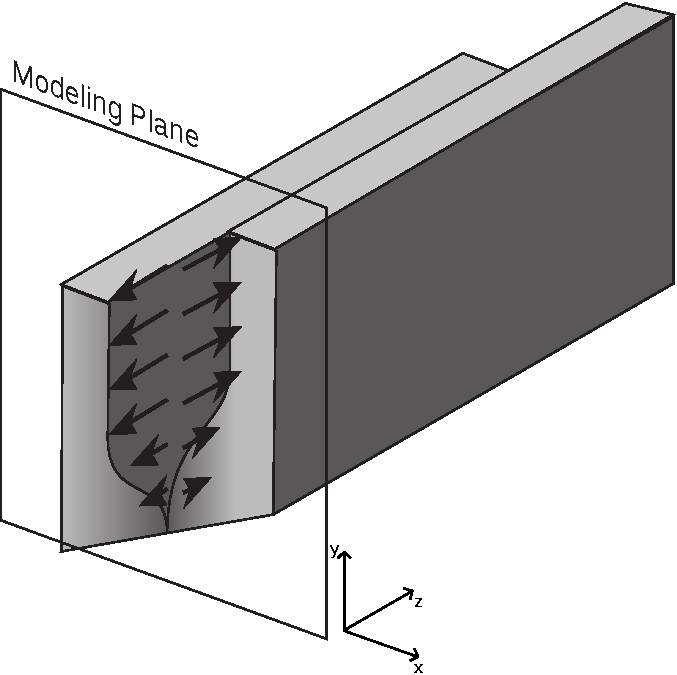
\includegraphics{aps}
\caption{Figure 1\-: Schematic representation of a fault and the modeled plane}
\end{DoxyImage}
 In this case, we can considered that displacement only occurs in the $z$ direction $ (u_{x}=u_{y}=0) $. Moreover, under this approximation no magnitude can vary along the $ z $ direction $(\frac{\partial}{\partial z}=0)$. Therefore, under this approximation $ \varepsilon_{xx} = \varepsilon_{yy} = \varepsilon_{zz} = \varepsilon_{xy} = \varepsilon_{yx}=0$, $\ast$ $ \varepsilon^v_{xx} = \varepsilon^v_{yy} = \varepsilon^v_{zz} = \varepsilon^v_{xy} = \varepsilon^v_{yx} = 0 $ and $ \sigma_{xx} = \sigma_{yy} = \sigma_{zz} = \sigma_{xy} = \sigma_{yx} = 0 $. In addition, we neglect the gravitational force. Therefore, the governing equations are reduced to\-:

\[ \partial_i \left( \mu \partial_i u_z \right) = f^v_z \]

where

\[ f^v_z(t_{n+1}) = \partial_i \left( 2\mu \varepsilon^v_{iz}(t_{n+1}) \right) = \partial_i \left[ 2 \mu \left(\varepsilon^v_{iz}(t_n) + \frac{\mu \Delta t_{n+1}}{2 * \eta} \partial_i u_z(t_n) \right) \right] \]\hypertarget{index_model}{}\section{Modeling}\label{index_model}
\hypertarget{index_setup}{}\subsection{Setup}\label{index_setup}
Here we will solve the visco-\/elastic equation in a two-\/dimensional domain of dimensions $a$ by $b$. We will solve for the displacement in the direction perpendicular to the plane $(u_z)$ caused by a fault also perpendicular to the modeled plane.

There are four possible boundary conditions\-:


\begin{DoxyItemize}
\item $\Gamma_0$ -\/ The locked part above the fault, with imposed zero displacement, $u_z=0$ (homogeneous Dirichlet boundary conditions).
\item $\Gamma_1$ -\/ Regions of imposed displacement, $u_z=U$ (non-\/homogeneous Dirichlet boundary conditions).
\item $\Gamma_2$ -\/ Zero tangential stress boundaries, $ n_i \sigma_{iz} = 0 $ (homogeneous Neumann boundary conditions).
\item $\Gamma_3$ -\/ Imposed tangential stress $ n_i \sigma_{iz} = S$ (non-\/homogeneous Neumann boundary conditions).
\end{DoxyItemize}\hypertarget{index_weak_form}{}\subsection{The Weak Form}\label{index_weak_form}
In order to solve the equation using the Finite Element Method we need to derive the weak form. We will begin with the partial differential equation that governs the dicplacement in a visco-\/elastic medium under the anti-\/plane shear approximation\-:

\[ \partial_i \left( \mu \partial_i u_z\right) = f^v_z \]

First we multiply the equation from the left by a test function $v$, and then we integrate over the whole domain\-:

\[ \int_{\Omega} v \cdot \partial_i \left( \mu \partial_i u_z \right) = \int_{\Omega} v \cdot \partial_i \left( 2 \mu \varepsilon^v_{iz} \right) \]

Integrating by parts both sides of the equation and using the Gauss theorem

\[ \int_{\Omega} \partial_i v \cdot \mu \partial_i u_z = \int_{\Omega} \partial_i v \cdot 2 \mu \varepsilon^v_{iz} + \int_{\partial \Omega} v \cdot \mu n_i \partial_i u_z - \int_{\partial \Omega} v \cdot n_i 2 \mu \varepsilon^v_{iz} \]

Considering that\-:

\[ \sigma_{iz} = 2 \mu \left( \varepsilon_{iz} - \varepsilon^v_{iz} \right) \]

The boundary term can be rewriten as\-:

\[ \int_{\Omega} \partial_i v \cdot \mu \partial_i u_z = \int_{\Omega} \partial_i v \cdot 2 \mu \varepsilon^v_{iz} + \int_{\partial \Omega} v \cdot n_i \sigma_{iz} \]

or\-:

\[ \left( \partial_i v, \mu \partial_i u_z \right)_{\Omega} = \left( \partial_i v, 2 \mu \varepsilon^v_{iz} \right)_{\Omega} + \left(v, n_i \sigma_{iz} \right)_{\partial \Omega} \]

where the operator $(a, b)$ is $ \int a \cdot b $.

In those boundaries where the displacement is imposed (Dirichlet boundary conditions), this is $\Gamma_0$ and $\Gamma_1$,the test function $v = 0$. The contribution of those boundaries in which the imposed tangential stress is zero (i.\-e., $\Gamma_2$) will not contribute to the right hand side either. On the other hand,those boundaries in which we impose a non-\/zero tangential stress (non-\/homogeneous Neumann boundary conditions), this is $\Gamma_3$, the test functions $v \neq 0$, and that part of the boundary integral has to be included in the weak form.

\[ \left( \partial_i v, \mu \partial_i u_z \right)_{\Omega} = \left( \partial_i v, 2 \mu \varepsilon^v_{iz} \right)_{\Omega} + \left(v, S \right)_{\Gamma^3} \]

where $S$ is the imposed tangential stress at the boundares $ \Gamma_3 $.

We can now replace the exact solution $ u_z $ for an approximate solution in terms of the shape functions, $ \sum_{k} U_k v_k(x_i) $. Here $U_k$ are the expansion coefficients we need to determine to find the approximate solution to the equation. Then, the problem is reduced to solving

\[AU=B\]

where the matrix A and the vector B are defined as\-:

\[A_{kl} = (\partial_i v_k, \mu \partial_i v_l)_{\Omega}\] \[B_k = (\partial_i v_k, 2 \mu \varepsilon^v_{iz})_\Omega + (v_k, S)_{\Gamma_3} \]

where $ k $ and $ l $ run through all the degrees of freedom.\hypertarget{index_adaptive_refinement}{}\subsection{Adaptive Mesh Refinement in Time Dependent Problems}\label{index_adaptive_refinement}
Every time step we need to use the solution and the viscous strain from the previous time step. The old solution is stored in a \href{https://www.dealii.org/8.4.0/doxygen/deal.II/classVector.html}{\tt Vector} with as many elements as the degrees of freedom the problem has, and is updated every time step. The old viscous strain is stored at each quadrature and can be accessed through a user pointer that each cell holds.

Every time the mesh is refined, the number of cells and degrees of freedom changes, therefore, as part of the mesh refinement we need to transfer the solution vector and the old viscous strain from the old mesh to the new one. For the solution vectors we just need to use \href{https://www.dealii.org/8.4.0/doxygen/deal.II/classSolutionTransfer.html}{\tt Solution\-Transfer} (see for example \href{https://www.dealii.org/8.2.0/doxygen/deal.II/step_26.html#codeHeatEquationrefine_meshcode}{\tt Step-\/26}). Transferring the old viscous strin is slightly more complicated, we first need to transfer the data stored in the quadrature points to a finite element field that is defined everywhere so that we can later transfer it to the new mesh (using \href{https://www.dealii.org/8.4.0/doxygen/deal.II/classSolutionTransfer.html}{\tt Solution\-Transfer} and then interpolate it to the new quadrature points. We need a discontinuous field that matches the values in the quadrature points (we will use a Discontinuous Galerking finite element \href{https://www.dealii.org/8.2.0/doxygen/deal.II/classFE__DGQ.html}{\tt F\-E\-\_\-\-D\-G\-Q}). 
\chapter{V\-E\-\_\-fault\-\_\-elastic}
\label{md_README}
\hypertarget{md_README}{}
\input{md_README}
\chapter{Namespace Index}
\section{Namespace List}
Here is a list of all namespaces with brief descriptions\-:\begin{DoxyCompactList}
\item\contentsline{section}{\hyperlink{namespacevsf}{vsf} }{\pageref{namespacevsf}}{}
\end{DoxyCompactList}

\chapter{Hierarchical Index}
\section{Class Hierarchy}
This inheritance list is sorted roughly, but not completely, alphabetically\-:\begin{DoxyCompactList}
\item Function\begin{DoxyCompactList}
\item \contentsline{section}{vsf\-:\-:Body\-Force$<$ dim $>$}{\pageref{classvsf_1_1BodyForce}}{}
\item \contentsline{section}{vsf\-:\-:Dirichlet\-\_\-\-B\-C$<$ dim $>$}{\pageref{classvsf_1_1Dirichlet__BC}}{}
\item \contentsline{section}{vsf\-:\-:Neumann\-\_\-\-B\-C$<$ dim $>$}{\pageref{classvsf_1_1Neumann__BC}}{}
\item \contentsline{section}{vsf\-:\-:Shear\-\_\-\-Modulus$<$ dim $>$}{\pageref{classvsf_1_1Shear__Modulus}}{}
\item \contentsline{section}{vsf\-:\-:Solution\-\_\-\-Savage$<$ dim $>$}{\pageref{classvsf_1_1Solution__Savage}}{}
\item \contentsline{section}{vsf\-:\-:Solution\-\_\-\-Turcotte$<$ dim $>$}{\pageref{classvsf_1_1Solution__Turcotte}}{}
\item \contentsline{section}{vsf\-:\-:Viscosity$<$ dim $>$}{\pageref{classvsf_1_1Viscosity}}{}
\end{DoxyCompactList}
\item \contentsline{section}{vsf\-:\-:Function\-Base$<$ dim $>$}{\pageref{classvsf_1_1FunctionBase}}{}
\begin{DoxyCompactList}
\item \contentsline{section}{vsf\-:\-:Ap\-Shear$<$ dim $>$}{\pageref{classvsf_1_1ApShear}}{}
\item \contentsline{section}{vsf\-:\-:Body\-Force$<$ dim $>$}{\pageref{classvsf_1_1BodyForce}}{}
\item \contentsline{section}{vsf\-:\-:Dirichlet\-\_\-\-B\-C$<$ dim $>$}{\pageref{classvsf_1_1Dirichlet__BC}}{}
\item \contentsline{section}{vsf\-:\-:Neumann\-\_\-\-B\-C$<$ dim $>$}{\pageref{classvsf_1_1Neumann__BC}}{}
\item \contentsline{section}{vsf\-:\-:Shear\-\_\-\-Modulus$<$ dim $>$}{\pageref{classvsf_1_1Shear__Modulus}}{}
\item \contentsline{section}{vsf\-:\-:Solution\-\_\-\-Savage$<$ dim $>$}{\pageref{classvsf_1_1Solution__Savage}}{}
\item \contentsline{section}{vsf\-:\-:Solution\-\_\-\-Turcotte$<$ dim $>$}{\pageref{classvsf_1_1Solution__Turcotte}}{}
\item \contentsline{section}{vsf\-:\-:Viscosity$<$ dim $>$}{\pageref{classvsf_1_1Viscosity}}{}
\end{DoxyCompactList}
\item \contentsline{section}{vsf\-:\-:Point\-History$<$ dim $>$}{\pageref{structvsf_1_1PointHistory}}{}
\end{DoxyCompactList}

\chapter{Class Index}
\section{Class List}
Here are the classes, structs, unions and interfaces with brief descriptions\-:\begin{DoxyCompactList}
\item\contentsline{section}{\hyperlink{classvsf_1_1ApShear}{vsf\-::\-Ap\-Shear$<$ dim $>$} }{\pageref{classvsf_1_1ApShear}}{}
\item\contentsline{section}{\hyperlink{classvsf_1_1BodyForce}{vsf\-::\-Body\-Force$<$ dim $>$} }{\pageref{classvsf_1_1BodyForce}}{}
\item\contentsline{section}{\hyperlink{classvsf_1_1Dirichlet__BC}{vsf\-::\-Dirichlet\-\_\-\-B\-C$<$ dim $>$} }{\pageref{classvsf_1_1Dirichlet__BC}}{}
\item\contentsline{section}{\hyperlink{classvsf_1_1FunctionBase}{vsf\-::\-Function\-Base$<$ dim $>$} }{\pageref{classvsf_1_1FunctionBase}}{}
\item\contentsline{section}{\hyperlink{classvsf_1_1Neumann__BC}{vsf\-::\-Neumann\-\_\-\-B\-C$<$ dim $>$} }{\pageref{classvsf_1_1Neumann__BC}}{}
\item\contentsline{section}{\hyperlink{structvsf_1_1PointHistory}{vsf\-::\-Point\-History$<$ dim $>$} }{\pageref{structvsf_1_1PointHistory}}{}
\item\contentsline{section}{\hyperlink{classvsf_1_1Shear__Modulus}{vsf\-::\-Shear\-\_\-\-Modulus$<$ dim $>$} }{\pageref{classvsf_1_1Shear__Modulus}}{}
\item\contentsline{section}{\hyperlink{classvsf_1_1Solution__Savage}{vsf\-::\-Solution\-\_\-\-Savage$<$ dim $>$} }{\pageref{classvsf_1_1Solution__Savage}}{}
\item\contentsline{section}{\hyperlink{classvsf_1_1Solution__Turcotte}{vsf\-::\-Solution\-\_\-\-Turcotte$<$ dim $>$} }{\pageref{classvsf_1_1Solution__Turcotte}}{}
\item\contentsline{section}{\hyperlink{classvsf_1_1Viscosity}{vsf\-::\-Viscosity$<$ dim $>$} }{\pageref{classvsf_1_1Viscosity}}{}
\end{DoxyCompactList}

\chapter{File Index}
\section{File List}
Here is a list of all files with brief descriptions\-:\begin{DoxyCompactList}
\item\contentsline{section}{\hyperlink{VE__fault__elastic_8cc}{V\-E\-\_\-fault\-\_\-elastic.\-cc} }{\pageref{VE__fault__elastic_8cc}}{}
\end{DoxyCompactList}

\chapter{Namespace Documentation}
\hypertarget{namespacevsf}{\section{vsf Namespace Reference}
\label{namespacevsf}\index{vsf@{vsf}}
}
\subsection*{Classes}
\begin{DoxyCompactItemize}
\item 
struct \hyperlink{structvsf_1_1PointHistory}{Point\-History}
\item 
class \hyperlink{classvsf_1_1FunctionBase}{Function\-Base}
\item 
class \hyperlink{classvsf_1_1Solution__Turcotte}{Solution\-\_\-\-Turcotte}
\item 
class \hyperlink{classvsf_1_1Solution__Savage}{Solution\-\_\-\-Savage}
\item 
class \hyperlink{classvsf_1_1Shear__Modulus}{Shear\-\_\-\-Modulus}
\item 
class \hyperlink{classvsf_1_1Viscosity}{Viscosity}
\item 
class \hyperlink{classvsf_1_1BodyForce}{Body\-Force}
\item 
class \hyperlink{classvsf_1_1Dirichlet__BC}{Dirichlet\-\_\-\-B\-C}
\item 
class \hyperlink{classvsf_1_1Neumann__BC}{Neumann\-\_\-\-B\-C}
\item 
class \hyperlink{classvsf_1_1ApShear}{Ap\-Shear}
\end{DoxyCompactItemize}

\chapter{Class Documentation}
\hypertarget{classvsf_1_1ApShear}{\section{vsf\-:\-:Ap\-Shear$<$ dim $>$ Class Template Reference}
\label{classvsf_1_1ApShear}\index{vsf\-::\-Ap\-Shear$<$ dim $>$@{vsf\-::\-Ap\-Shear$<$ dim $>$}}
}
Inheritance diagram for vsf\-:\-:Ap\-Shear$<$ dim $>$\-:\begin{figure}[H]
\begin{center}
\leavevmode
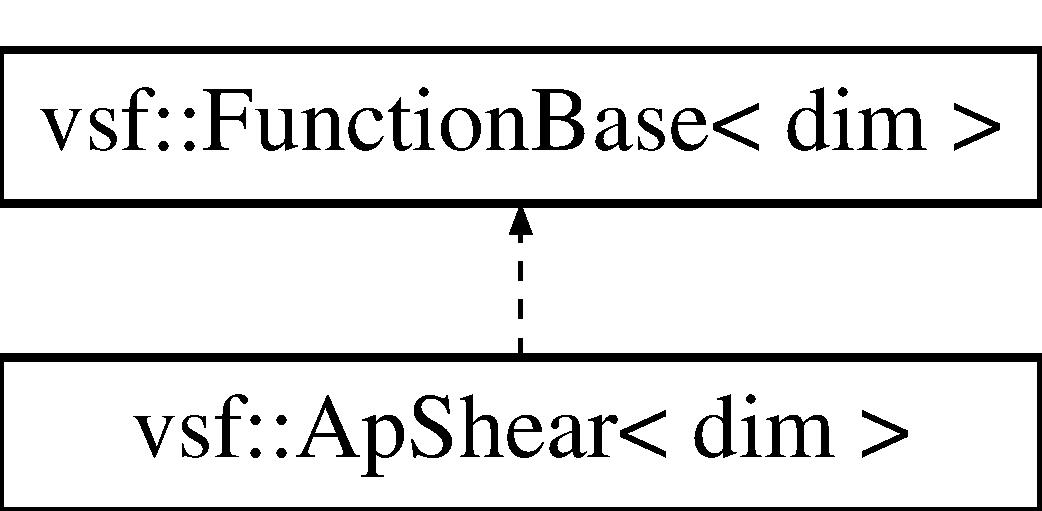
\includegraphics[height=2.000000cm]{classvsf_1_1ApShear}
\end{center}
\end{figure}
\subsection*{Public Types}
\begin{DoxyCompactItemize}
\item 
enum \hyperlink{classvsf_1_1ApShear_aef8049bf5f942237a19e8b88ddc19e8c}{Refinement\-Mode} \{ \hyperlink{classvsf_1_1ApShear_aef8049bf5f942237a19e8b88ddc19e8ca4d42958e34994e37831e0e390b554a22}{global\-\_\-refinement}, 
\hyperlink{classvsf_1_1ApShear_aef8049bf5f942237a19e8b88ddc19e8ca6d458d887ac9b2cdfc9bdf078a2d0f78}{adaptive\-\_\-refinement}
 \}
\item 
enum \hyperlink{classvsf_1_1ApShear_a354ce33d5e60761e975bdb924119354d}{Model} \{ \hyperlink{classvsf_1_1ApShear_a354ce33d5e60761e975bdb924119354dab1d7d25f092b95270851c3cf1faa7bb5}{turcotte}, 
\hyperlink{classvsf_1_1ApShear_a354ce33d5e60761e975bdb924119354da218f8a8439447f9d74a62070ad9086dc}{savage}
 \}
\end{DoxyCompactItemize}
\subsection*{Public Member Functions}
\begin{DoxyCompactItemize}
\item 
\hyperlink{classvsf_1_1ApShear_a58df51f254eb8ea07f1523c0d76246fc}{Ap\-Shear} (const Finite\-Element$<$ dim $>$ \&\hyperlink{classvsf_1_1ApShear_a228388a897a688b79d0800f3bb18697f}{fe}, const Finite\-Element$<$ dim $>$ \&\hyperlink{classvsf_1_1ApShear_a3c2f9d0e479ed2ebcb3660a3b7b72aee}{history\-\_\-fe}, const unsigned int \hyperlink{classvsf_1_1ApShear_ae4927f95e4a98c107d743a078a9b1bc8}{degree}, const \hyperlink{classvsf_1_1ApShear_aef8049bf5f942237a19e8b88ddc19e8c}{Refinement\-Mode} \hyperlink{classvsf_1_1ApShear_a523d3e34e242a9dbcf1d727dc17874b6}{refinement\-\_\-mode}, const \hyperlink{classvsf_1_1ApShear_a354ce33d5e60761e975bdb924119354d}{Model} \hyperlink{classvsf_1_1ApShear_a3a6fb4045df9297aea20326cb0df5748}{model})
\item 
\hyperlink{classvsf_1_1ApShear_a7d7cb7564f9d34ccd1a9d4183225cab7}{$\sim$\-Ap\-Shear} ()
\item 
void \hyperlink{classvsf_1_1ApShear_a8c366c00d028013a6949ee94786038ac}{run} ()
\end{DoxyCompactItemize}
\subsection*{Private Member Functions}
\begin{DoxyCompactItemize}
\item 
void \hyperlink{classvsf_1_1ApShear_a49ba2c773ca4f6a1946dee0d08e76901}{do\-\_\-first\-\_\-time\-\_\-step} ()
\item 
void \hyperlink{classvsf_1_1ApShear_a230bde382d9f71b56181ae943634611e}{do\-\_\-time\-\_\-step} ()
\item 
void \hyperlink{classvsf_1_1ApShear_ab12b87e8d50262d7735c5ba0aab1549f}{make\-\_\-grid\-\_\-turcotte} ()
\item 
void \hyperlink{classvsf_1_1ApShear_a265e55ba004056c96ab59aa633d5510f}{make\-\_\-grid\-\_\-savage} ()
\item 
void \hyperlink{classvsf_1_1ApShear_ae0c1413d01e98526e4a61a7324bf2ae0}{refine\-\_\-grid} (const unsigned int min\-\_\-grid\-\_\-level, const unsigned int max\-\_\-grid\-\_\-level)
\item 
void \hyperlink{classvsf_1_1ApShear_ad0d3a17afc6092f53560a50fd21c82f3}{qpoints\-\_\-to\-\_\-\-D\-G} ()
\item 
void \hyperlink{classvsf_1_1ApShear_accf1d57fc6f81758bf06a93ef70f74c4}{D\-G\-\_\-to\-\_\-qpoints} ()
\item 
void \hyperlink{classvsf_1_1ApShear_aa64a11292b5664242bb982a1a400fae0}{setup\-\_\-system} ()
\item 
void \hyperlink{classvsf_1_1ApShear_a7e74ebe08f8b6586a71c606a64ab4db4}{setup\-\_\-quadrature\-\_\-point\-\_\-history} ()
\item 
void \hyperlink{classvsf_1_1ApShear_a6b2acd54f930d5deac94064923e1aa7b}{update\-\_\-quadrature\-\_\-point\-\_\-history} ()
\item 
void \hyperlink{classvsf_1_1ApShear_a53c9284a86fc90a817ddad24eaf18569}{assemble\-\_\-system} ()
\item 
void \hyperlink{classvsf_1_1ApShear_a7e90fa26f6c78252f8e4592d5fc7adcf}{solve} ()
\item 
void \hyperlink{classvsf_1_1ApShear_ab58464c123140aaa9e231ddea2e94a03}{get\-\_\-time\-\_\-step} ()
\item 
void \hyperlink{classvsf_1_1ApShear_aa7a681d59cd2147f021245e7cccc0d32}{compare\-\_\-solutions\-\_\-turcotte} ()
\item 
void \hyperlink{classvsf_1_1ApShear_a2b1bb3ca132f62ccf3c2ca1e4e81f97c}{compare\-\_\-solutions\-\_\-savage} ()
\item 
void \hyperlink{classvsf_1_1ApShear_af10b1bbda00ef235b3bff742831890bf}{output\-\_\-results} ()
\end{DoxyCompactItemize}
\subsection*{Private Attributes}
\begin{DoxyCompactItemize}
\item 
const unsigned int \hyperlink{classvsf_1_1ApShear_ae4927f95e4a98c107d743a078a9b1bc8}{degree}
\item 
Triangulation$<$ dim $>$ \hyperlink{classvsf_1_1ApShear_a53d0e9d3fdabcac44cc7c6408ace451b}{triangulation}
\item 
Do\-F\-Handler$<$ dim $>$ \hyperlink{classvsf_1_1ApShear_a55da0ced5f7ee7c16a518073f4524ffb}{dof\-\_\-handler}
\item 
Do\-F\-Handler$<$ dim $>$ \hyperlink{classvsf_1_1ApShear_acdcfb9ec77c56722ce42173f7599c336}{history\-\_\-dof\-\_\-handler}
\item 
const Q\-Gauss$<$ dim $>$ \hyperlink{classvsf_1_1ApShear_a2926794d4cbeed7550443a4999868110}{quadrature\-\_\-formula}
\item 
Smart\-Pointer$<$ const \\*
Finite\-Element$<$ dim $>$ $>$ \hyperlink{classvsf_1_1ApShear_a228388a897a688b79d0800f3bb18697f}{fe}
\item 
Smart\-Pointer$<$ const \\*
Finite\-Element$<$ dim $>$ $>$ \hyperlink{classvsf_1_1ApShear_a3c2f9d0e479ed2ebcb3660a3b7b72aee}{history\-\_\-fe}
\item 
Constraint\-Matrix \hyperlink{classvsf_1_1ApShear_afcd25b4c0be9a4c7e69165e6eb151240}{constraints}
\item 
Sparsity\-Pattern \hyperlink{classvsf_1_1ApShear_a065cb85ed84df073fd1b726667eebcc3}{sparsity\-\_\-pattern}
\item 
Sparse\-Matrix$<$ double $>$ \hyperlink{classvsf_1_1ApShear_a8735861f0a5530262407cd52b7a1b386}{system\-\_\-matrix}
\item 
Vector$<$ double $>$ \hyperlink{classvsf_1_1ApShear_ab1046cf38cb6535dd0ab78793bccf6a1}{system\-\_\-rhs}
\item 
Vector$<$ double $>$ \hyperlink{classvsf_1_1ApShear_ae4ee8cb26cbb92aa25fa91d2eb2198db}{solution}
\item 
std\-::vector$<$ \hyperlink{structvsf_1_1PointHistory}{Point\-History}$<$ dim $>$ $>$ \hyperlink{classvsf_1_1ApShear_aeb702a26aef2b0a7d0d27d46909b81b9}{quadrature\-\_\-point\-\_\-history}
\item 
std\-::vector$<$ Vector$<$ double $>$ $>$ \hyperlink{classvsf_1_1ApShear_ab47e19f00b1a5475699673c44d48ab8d}{history\-\_\-field}
\item 
const \hyperlink{classvsf_1_1ApShear_aef8049bf5f942237a19e8b88ddc19e8c}{Refinement\-Mode} \hyperlink{classvsf_1_1ApShear_a523d3e34e242a9dbcf1d727dc17874b6}{refinement\-\_\-mode}
\item 
const \hyperlink{classvsf_1_1ApShear_a354ce33d5e60761e975bdb924119354d}{Model} \hyperlink{classvsf_1_1ApShear_a3a6fb4045df9297aea20326cb0df5748}{model}
\item 
const unsigned int \hyperlink{classvsf_1_1ApShear_ab02322073eb961685e8daef27729bf8d}{n\-\_\-initial\-\_\-global\-\_\-refinement}
\item 
const unsigned int \hyperlink{classvsf_1_1ApShear_a5c702ecbc19d28d835e666c8ee87c4eb}{n\-\_\-pre\-\_\-refinment}
\item 
unsigned int \hyperlink{classvsf_1_1ApShear_aa8a20bee076f8edea5090fe587af2630}{step}
\item 
double \hyperlink{classvsf_1_1ApShear_ab11c93d8c80fc10976c8fb91a733cf92}{time\-\_\-step}
\item 
double \hyperlink{classvsf_1_1ApShear_ab4bd5313e37b8819910d35aaae0a2373}{total\-\_\-time}
\item 
std\-::vector$<$ double $>$ \hyperlink{classvsf_1_1ApShear_a9aec407d8269d51336f50f3a9d94b53b}{surface\-\_\-q\-\_\-points}
\item 
std\-::vector$<$ double $>$ \hyperlink{classvsf_1_1ApShear_a96a76f66c7155491bfe3d3c50d576fe9}{surface\-\_\-analytical\-\_\-solution}
\item 
std\-::vector$<$ double $>$ \hyperlink{classvsf_1_1ApShear_adbc4b0f8e2a3282b27241a2088f9717d}{surface\-\_\-numerical\-\_\-solution}
\item 
double \hyperlink{classvsf_1_1ApShear_a980e61d73be5cae2b8e8498b9ffc087a}{error}
\end{DoxyCompactItemize}
\subsection*{Additional Inherited Members}


\subsection{Detailed Description}
\subsubsection*{template$<$int dim$>$class vsf\-::\-Ap\-Shear$<$ dim $>$}

The main class of the code, contains all the functions that do the job of setting up and solving the model.

\begin{DoxyNote}{Note}
Since the model parameters have been set in \hyperlink{classvsf_1_1FunctionBase}{Function\-Base}, this new class will also inherit from it. 
\end{DoxyNote}


\subsection{Member Enumeration Documentation}
\hypertarget{classvsf_1_1ApShear_a354ce33d5e60761e975bdb924119354d}{\index{vsf\-::\-Ap\-Shear@{vsf\-::\-Ap\-Shear}!Model@{Model}}
\index{Model@{Model}!vsf::ApShear@{vsf\-::\-Ap\-Shear}}
\subsubsection[{Model}]{\setlength{\rightskip}{0pt plus 5cm}template$<$int dim$>$ enum {\bf vsf\-::\-Ap\-Shear\-::\-Model}}}\label{classvsf_1_1ApShear_a354ce33d5e60761e975bdb924119354d}
\begin{Desc}
\item[Enumerator]\par
\begin{description}
\index{turcotte@{turcotte}!vsf\-::\-Ap\-Shear@{vsf\-::\-Ap\-Shear}}\index{vsf\-::\-Ap\-Shear@{vsf\-::\-Ap\-Shear}!turcotte@{turcotte}}\item[{\em 
\hypertarget{classvsf_1_1ApShear_a354ce33d5e60761e975bdb924119354dab1d7d25f092b95270851c3cf1faa7bb5}{turcotte}\label{classvsf_1_1ApShear_a354ce33d5e60761e975bdb924119354dab1d7d25f092b95270851c3cf1faa7bb5}
}]\index{savage@{savage}!vsf\-::\-Ap\-Shear@{vsf\-::\-Ap\-Shear}}\index{vsf\-::\-Ap\-Shear@{vsf\-::\-Ap\-Shear}!savage@{savage}}\item[{\em 
\hypertarget{classvsf_1_1ApShear_a354ce33d5e60761e975bdb924119354da218f8a8439447f9d74a62070ad9086dc}{savage}\label{classvsf_1_1ApShear_a354ce33d5e60761e975bdb924119354da218f8a8439447f9d74a62070ad9086dc}
}]\end{description}
\end{Desc}
\hypertarget{classvsf_1_1ApShear_aef8049bf5f942237a19e8b88ddc19e8c}{\index{vsf\-::\-Ap\-Shear@{vsf\-::\-Ap\-Shear}!Refinement\-Mode@{Refinement\-Mode}}
\index{Refinement\-Mode@{Refinement\-Mode}!vsf::ApShear@{vsf\-::\-Ap\-Shear}}
\subsubsection[{Refinement\-Mode}]{\setlength{\rightskip}{0pt plus 5cm}template$<$int dim$>$ enum {\bf vsf\-::\-Ap\-Shear\-::\-Refinement\-Mode}}}\label{classvsf_1_1ApShear_aef8049bf5f942237a19e8b88ddc19e8c}
\begin{Desc}
\item[Enumerator]\par
\begin{description}
\index{global\-\_\-refinement@{global\-\_\-refinement}!vsf\-::\-Ap\-Shear@{vsf\-::\-Ap\-Shear}}\index{vsf\-::\-Ap\-Shear@{vsf\-::\-Ap\-Shear}!global\-\_\-refinement@{global\-\_\-refinement}}\item[{\em 
\hypertarget{classvsf_1_1ApShear_aef8049bf5f942237a19e8b88ddc19e8ca4d42958e34994e37831e0e390b554a22}{global\-\_\-refinement}\label{classvsf_1_1ApShear_aef8049bf5f942237a19e8b88ddc19e8ca4d42958e34994e37831e0e390b554a22}
}]\index{adaptive\-\_\-refinement@{adaptive\-\_\-refinement}!vsf\-::\-Ap\-Shear@{vsf\-::\-Ap\-Shear}}\index{vsf\-::\-Ap\-Shear@{vsf\-::\-Ap\-Shear}!adaptive\-\_\-refinement@{adaptive\-\_\-refinement}}\item[{\em 
\hypertarget{classvsf_1_1ApShear_aef8049bf5f942237a19e8b88ddc19e8ca6d458d887ac9b2cdfc9bdf078a2d0f78}{adaptive\-\_\-refinement}\label{classvsf_1_1ApShear_aef8049bf5f942237a19e8b88ddc19e8ca6d458d887ac9b2cdfc9bdf078a2d0f78}
}]\end{description}
\end{Desc}


\subsection{Constructor \& Destructor Documentation}
\hypertarget{classvsf_1_1ApShear_a58df51f254eb8ea07f1523c0d76246fc}{\index{vsf\-::\-Ap\-Shear@{vsf\-::\-Ap\-Shear}!Ap\-Shear@{Ap\-Shear}}
\index{Ap\-Shear@{Ap\-Shear}!vsf::ApShear@{vsf\-::\-Ap\-Shear}}
\subsubsection[{Ap\-Shear}]{\setlength{\rightskip}{0pt plus 5cm}template$<$int dim$>$ {\bf vsf\-::\-Ap\-Shear}$<$ dim $>$\-::{\bf Ap\-Shear} (
\begin{DoxyParamCaption}
\item[{const Finite\-Element$<$ dim $>$ \&}]{fe, }
\item[{const Finite\-Element$<$ dim $>$ \&}]{history\-\_\-fe, }
\item[{const unsigned int}]{degree, }
\item[{const {\bf Refinement\-Mode}}]{refinement\-\_\-mode, }
\item[{const {\bf Model}}]{model}
\end{DoxyParamCaption}
)}}\label{classvsf_1_1ApShear_a58df51f254eb8ea07f1523c0d76246fc}

\begin{DoxyParams}{Parameters}
{\em fe} & The code is written so different elements can be used and are defined as input parameters. \\
\hline
{\em history\-\_\-fe} & F\-E to store history data \\
\hline
{\em degree} & To be consistent, we define the degree of the finite elements as an input parameter. \\
\hline
{\em refinement\-\_\-mode} & The mesh can be refined either globally (global\-\_\-refinement) or adaptively (adaptive\-\_\-refinement), which one to use is defined as an input parameters \\
\hline
{\em model} & The code can be used to simmulate the deformation caused by a fault using two models. \\
\hline
\end{DoxyParams}
\hypertarget{classvsf_1_1ApShear_a7d7cb7564f9d34ccd1a9d4183225cab7}{\index{vsf\-::\-Ap\-Shear@{vsf\-::\-Ap\-Shear}!$\sim$\-Ap\-Shear@{$\sim$\-Ap\-Shear}}
\index{$\sim$\-Ap\-Shear@{$\sim$\-Ap\-Shear}!vsf::ApShear@{vsf\-::\-Ap\-Shear}}
\subsubsection[{$\sim$\-Ap\-Shear}]{\setlength{\rightskip}{0pt plus 5cm}template$<$int dim$>$ {\bf vsf\-::\-Ap\-Shear}$<$ dim $>$\-::$\sim${\bf Ap\-Shear} (
\begin{DoxyParamCaption}
{}
\end{DoxyParamCaption}
)}}\label{classvsf_1_1ApShear_a7d7cb7564f9d34ccd1a9d4183225cab7}


\subsection{Member Function Documentation}
\hypertarget{classvsf_1_1ApShear_a53c9284a86fc90a817ddad24eaf18569}{\index{vsf\-::\-Ap\-Shear@{vsf\-::\-Ap\-Shear}!assemble\-\_\-system@{assemble\-\_\-system}}
\index{assemble\-\_\-system@{assemble\-\_\-system}!vsf::ApShear@{vsf\-::\-Ap\-Shear}}
\subsubsection[{assemble\-\_\-system}]{\setlength{\rightskip}{0pt plus 5cm}template$<$int dim$>$ void {\bf vsf\-::\-Ap\-Shear}$<$ dim $>$\-::assemble\-\_\-system (
\begin{DoxyParamCaption}
{}
\end{DoxyParamCaption}
)\hspace{0.3cm}{\ttfamily [private]}}}\label{classvsf_1_1ApShear_a53c9284a86fc90a817ddad24eaf18569}
Assemble stiffness matrix and R\-H\-S.

The stiffness matrix and R\-H\-S are assembled here. To assemble the stiffness matrix and R\-H\-S for the given problem we assemble the local matrices for each element and the transfer it to the global matrix.

Apply homogeneous Neumann boundary conditions. We loop over all the faces in each cell. We check if that face is in a boundary and if it is a boundary of type 3 (non-\/homogeneous Neumann boundary conditions), to those faces we add the corresponing contribution.\hypertarget{classvsf_1_1ApShear_a2b1bb3ca132f62ccf3c2ca1e4e81f97c}{\index{vsf\-::\-Ap\-Shear@{vsf\-::\-Ap\-Shear}!compare\-\_\-solutions\-\_\-savage@{compare\-\_\-solutions\-\_\-savage}}
\index{compare\-\_\-solutions\-\_\-savage@{compare\-\_\-solutions\-\_\-savage}!vsf::ApShear@{vsf\-::\-Ap\-Shear}}
\subsubsection[{compare\-\_\-solutions\-\_\-savage}]{\setlength{\rightskip}{0pt plus 5cm}template$<$int dim$>$ void {\bf vsf\-::\-Ap\-Shear}$<$ dim $>$\-::compare\-\_\-solutions\-\_\-savage (
\begin{DoxyParamCaption}
{}
\end{DoxyParamCaption}
)\hspace{0.3cm}{\ttfamily [private]}}}\label{classvsf_1_1ApShear_a2b1bb3ca132f62ccf3c2ca1e4e81f97c}
The numerical solution is compared against Savage and Burford Model

This function will take care of computing and storing the difference between the numerical solution and the analytical solution from Turcotte and Spence Model \cite{turcotte_spence_74}. At the end we will output the results in several graphs. The comparison will stored in three different variables\-:
\begin{DoxyItemize}
\item analytical\-\_\-solution\-: Analytical solution computed at each quadrature point of the final mesh.
\item surface\-\_\-numerical\-\_\-solution\-: Numerical solution in each quadrature point at each refinement cycle.
\item integrated\-\_\-diff\-: Integrated difference between both solutions using the L1 norm. 
\end{DoxyItemize}First we need to run a loop over every cell and every quadrature point to determine if they are located at the surface, if so, we will compute the analytical solution and extract the numerical solution to store them in analytical\-\_\-solution and numerical\-\_\-solution. Once we have both solutions at the surface, we will compute the integrated difference between them and we will store it in integrated\-\_\-diff.\hypertarget{classvsf_1_1ApShear_aa7a681d59cd2147f021245e7cccc0d32}{\index{vsf\-::\-Ap\-Shear@{vsf\-::\-Ap\-Shear}!compare\-\_\-solutions\-\_\-turcotte@{compare\-\_\-solutions\-\_\-turcotte}}
\index{compare\-\_\-solutions\-\_\-turcotte@{compare\-\_\-solutions\-\_\-turcotte}!vsf::ApShear@{vsf\-::\-Ap\-Shear}}
\subsubsection[{compare\-\_\-solutions\-\_\-turcotte}]{\setlength{\rightskip}{0pt plus 5cm}template$<$int dim$>$ void {\bf vsf\-::\-Ap\-Shear}$<$ dim $>$\-::compare\-\_\-solutions\-\_\-turcotte (
\begin{DoxyParamCaption}
{}
\end{DoxyParamCaption}
)\hspace{0.3cm}{\ttfamily [private]}}}\label{classvsf_1_1ApShear_aa7a681d59cd2147f021245e7cccc0d32}
The numerical solution is compared against Turcotte and Spence Model

This function will take care of computing and storing the difference between the numerical solution and the analytical solution from Turcotte and Spence Model \cite{turcotte_spence_74}. At the end we will output the results in several graphs. The comparison will stored in three different variables\-:
\begin{DoxyItemize}
\item analytical\-\_\-solution\-: Analytical solution computed at each quadrature point of the final mesh.
\item surface\-\_\-numerical\-\_\-solution\-: Numerical solution in each quadrature point at each refinement cycle.
\item integrated\-\_\-diff\-: Integrated difference between both solutions using the L1 norm. 
\end{DoxyItemize}First we need to run a loop over every cell and every quadrature point to determine if they are located at the surface, if so, we will compute the analytical solution and extract the numerical solution to store them in analytical\-\_\-solution and numerical\-\_\-solution. Once we have both solutions at the surface, we will compute the integrated difference between them and we will store it in integrated\-\_\-diff.\hypertarget{classvsf_1_1ApShear_accf1d57fc6f81758bf06a93ef70f74c4}{\index{vsf\-::\-Ap\-Shear@{vsf\-::\-Ap\-Shear}!D\-G\-\_\-to\-\_\-qpoints@{D\-G\-\_\-to\-\_\-qpoints}}
\index{D\-G\-\_\-to\-\_\-qpoints@{D\-G\-\_\-to\-\_\-qpoints}!vsf::ApShear@{vsf\-::\-Ap\-Shear}}
\subsubsection[{D\-G\-\_\-to\-\_\-qpoints}]{\setlength{\rightskip}{0pt plus 5cm}template$<$int dim$>$ void {\bf vsf\-::\-Ap\-Shear}$<$ dim $>$\-::D\-G\-\_\-to\-\_\-qpoints (
\begin{DoxyParamCaption}
{}
\end{DoxyParamCaption}
)\hspace{0.3cm}{\ttfamily [private]}}}\label{classvsf_1_1ApShear_accf1d57fc6f81758bf06a93ef70f74c4}
The information stored in a Discontinious Galerking space is moved to the quadrature points

After the mesh has been refined, we need to transfer the viscous strain back to the quadrature points. For more details see \href{https://www.dealii.org/8.2.0/doxygen/deal.II/step_18.html#Refinementduringtimesteps}{\tt Step-\/18} \hypertarget{classvsf_1_1ApShear_a49ba2c773ca4f6a1946dee0d08e76901}{\index{vsf\-::\-Ap\-Shear@{vsf\-::\-Ap\-Shear}!do\-\_\-first\-\_\-time\-\_\-step@{do\-\_\-first\-\_\-time\-\_\-step}}
\index{do\-\_\-first\-\_\-time\-\_\-step@{do\-\_\-first\-\_\-time\-\_\-step}!vsf::ApShear@{vsf\-::\-Ap\-Shear}}
\subsubsection[{do\-\_\-first\-\_\-time\-\_\-step}]{\setlength{\rightskip}{0pt plus 5cm}template$<$int dim$>$ void {\bf vsf\-::\-Ap\-Shear}$<$ dim $>$\-::do\-\_\-first\-\_\-time\-\_\-step (
\begin{DoxyParamCaption}
{}
\end{DoxyParamCaption}
)\hspace{0.3cm}{\ttfamily [private]}}}\label{classvsf_1_1ApShear_a49ba2c773ca4f6a1946dee0d08e76901}
Create the initial mesh and perform preliminary refinements and solve for the initial time step

In the first time step we will create a uniform grid and set the boundary conditions depending on the model that we want to solve. Then we will solve the problem and refine the mesh adaptively several times \hypertarget{classvsf_1_1ApShear_a230bde382d9f71b56181ae943634611e}{\index{vsf\-::\-Ap\-Shear@{vsf\-::\-Ap\-Shear}!do\-\_\-time\-\_\-step@{do\-\_\-time\-\_\-step}}
\index{do\-\_\-time\-\_\-step@{do\-\_\-time\-\_\-step}!vsf::ApShear@{vsf\-::\-Ap\-Shear}}
\subsubsection[{do\-\_\-time\-\_\-step}]{\setlength{\rightskip}{0pt plus 5cm}template$<$int dim$>$ void {\bf vsf\-::\-Ap\-Shear}$<$ dim $>$\-::do\-\_\-time\-\_\-step (
\begin{DoxyParamCaption}
{}
\end{DoxyParamCaption}
)\hspace{0.3cm}{\ttfamily [private]}}}\label{classvsf_1_1ApShear_a230bde382d9f71b56181ae943634611e}
Solve for successive time steps (includes mesh refinement every several time steps).

In successive time steps we will update the viscous strain (using the solution and the viscous strain from the last time step) and we will solve again. The mesh will be refined adaptively every several time steps. \hypertarget{classvsf_1_1ApShear_ab58464c123140aaa9e231ddea2e94a03}{\index{vsf\-::\-Ap\-Shear@{vsf\-::\-Ap\-Shear}!get\-\_\-time\-\_\-step@{get\-\_\-time\-\_\-step}}
\index{get\-\_\-time\-\_\-step@{get\-\_\-time\-\_\-step}!vsf::ApShear@{vsf\-::\-Ap\-Shear}}
\subsubsection[{get\-\_\-time\-\_\-step}]{\setlength{\rightskip}{0pt plus 5cm}template$<$int dim$>$ void {\bf vsf\-::\-Ap\-Shear}$<$ dim $>$\-::get\-\_\-time\-\_\-step (
\begin{DoxyParamCaption}
{}
\end{DoxyParamCaption}
)\hspace{0.3cm}{\ttfamily [private]}}}\label{classvsf_1_1ApShear_ab58464c123140aaa9e231ddea2e94a03}
Obtain the the time step increase

We need to calculate the size of each time step. We choose a size such that, the algorithm is stable \cite{cormeau_75} \cite{yamasaki_houseman_12:}

\[ \Delta t = \frac{\eta}{24 \mu} \]

We use the minimum value of $ \Delta t $ in the whole domain. Therefore, we need to compute the time increment at every quadrature point.

\begin{DoxyNote}{Note}
In the current implementation, both the shear modulus and the viscosity are uniform, and so will be the time step increment. However, we will still calculate the time step increment at every point, so it is easier to implement non-\/uniform parameters in the future. 
\end{DoxyNote}
\hypertarget{classvsf_1_1ApShear_a265e55ba004056c96ab59aa633d5510f}{\index{vsf\-::\-Ap\-Shear@{vsf\-::\-Ap\-Shear}!make\-\_\-grid\-\_\-savage@{make\-\_\-grid\-\_\-savage}}
\index{make\-\_\-grid\-\_\-savage@{make\-\_\-grid\-\_\-savage}!vsf::ApShear@{vsf\-::\-Ap\-Shear}}
\subsubsection[{make\-\_\-grid\-\_\-savage}]{\setlength{\rightskip}{0pt plus 5cm}template$<$int dim$>$ void {\bf vsf\-::\-Ap\-Shear}$<$ dim $>$\-::make\-\_\-grid\-\_\-savage (
\begin{DoxyParamCaption}
{}
\end{DoxyParamCaption}
)\hspace{0.3cm}{\ttfamily [private]}}}\label{classvsf_1_1ApShear_a265e55ba004056c96ab59aa633d5510f}
Create initial mesh by refining globally several times. Prepare boundaries for Savage and Burford Model

The initial mesh will consist of regular rectangular elements. This mesh will be refined in successive steps using \hyperlink{classvsf_1_1ApShear_ae0c1413d01e98526e4a61a7324bf2ae0}{refine\-\_\-grid()}. First a mesh is created with elements of the highest possible quality (as close to square as possible). Then this mesh is refined globally a given number of times.

\begin{DoxyNote}{Note}
If the fault is very small it can be ignored (if it's size is smaller than the element size). If this happens, include more global refinement steps. 
\end{DoxyNote}
Once the mesh has been created and refined, we assign an indicator to each part of the boundary, depending on what kind of boundary it is. There are four possible boundary conditions\-:


\begin{DoxyItemize}
\item 0) The locked part above the fault, with imposed zero displacement (homogeneous Dirichlet boundary conditions).
\item 1) Regions of imposed displacement (non-\/homogeneous Dirichlet boundary conditions).
\item 2) Free boundaries, with zero imposed stress (homogeneous Neumann boundary conditions).
\item 3) Imposed stress (non-\/homogeneous boundary conditions.

For Savage and Burford model \cite{savage_burford_73}, the locked part (0) will be on the left boundary, from the top to a certain depth $d$. From that depth until the bottom of the model we impose a displacement $UD$ (1). The bottom boundary will have the same imposed displacement (1). Finally, the top and left boundaries will be free (2).
\end{DoxyItemize}\hypertarget{classvsf_1_1ApShear_ab12b87e8d50262d7735c5ba0aab1549f}{\index{vsf\-::\-Ap\-Shear@{vsf\-::\-Ap\-Shear}!make\-\_\-grid\-\_\-turcotte@{make\-\_\-grid\-\_\-turcotte}}
\index{make\-\_\-grid\-\_\-turcotte@{make\-\_\-grid\-\_\-turcotte}!vsf::ApShear@{vsf\-::\-Ap\-Shear}}
\subsubsection[{make\-\_\-grid\-\_\-turcotte}]{\setlength{\rightskip}{0pt plus 5cm}template$<$int dim$>$ void {\bf vsf\-::\-Ap\-Shear}$<$ dim $>$\-::make\-\_\-grid\-\_\-turcotte (
\begin{DoxyParamCaption}
{}
\end{DoxyParamCaption}
)\hspace{0.3cm}{\ttfamily [private]}}}\label{classvsf_1_1ApShear_ab12b87e8d50262d7735c5ba0aab1549f}
Create initial mesh by refining globally several times. Prepare boundaries for Turcotte and Spence Model

The initial mesh will consist of regular rectangular elements. This mesh will be refined in successive steps using \hyperlink{classvsf_1_1ApShear_ae0c1413d01e98526e4a61a7324bf2ae0}{refine\-\_\-grid()}. First a mesh is created with elements of the highest possible quality (as close to square as possible). Then this mesh is refined globally a given number of times.

\begin{DoxyNote}{Note}
If the fault is very small it may be ignored (if it's size is smaller than the element size). If this happens, include more global refinement steps. 
\end{DoxyNote}
Once the mesh has been created and refined, we assign an indicator to each part of the boundary, depending on what kind of boundary it is. There are four possible boundary conditions\-:


\begin{DoxyItemize}
\item 0) The locked part above the fault, with imposed zero displacement (homogeneous Dirichlet boundary conditions).
\item 1) Regions of imposed displacement (non-\/homogeneous Dirichlet boundary conditions).
\item 2) Free boundaries, with zero imposed stress (homogeneous Neumann boundary conditions).
\item 3) Imposed stress (non-\/homogeneous boundary conditions.

For Turcotte and Spence's model \cite{turcotte_spence_74}, the locked part (0) will be on the left boundary, from the top to a certain depth $d$. From that depth until the bottom of the model the boundary will be free (2). The top and bottom boundaries will also be free (2). Finally, the leftmost boundary will have an imposed stress $S$ (3).
\end{DoxyItemize}\hypertarget{classvsf_1_1ApShear_af10b1bbda00ef235b3bff742831890bf}{\index{vsf\-::\-Ap\-Shear@{vsf\-::\-Ap\-Shear}!output\-\_\-results@{output\-\_\-results}}
\index{output\-\_\-results@{output\-\_\-results}!vsf::ApShear@{vsf\-::\-Ap\-Shear}}
\subsubsection[{output\-\_\-results}]{\setlength{\rightskip}{0pt plus 5cm}template$<$int dim$>$ void {\bf vsf\-::\-Ap\-Shear}$<$ dim $>$\-::output\-\_\-results (
\begin{DoxyParamCaption}
{}
\end{DoxyParamCaption}
)\hspace{0.3cm}{\ttfamily [private]}}}\label{classvsf_1_1ApShear_af10b1bbda00ef235b3bff742831890bf}
The results will be output in this step. Three different outputs are generated.
\begin{DoxyItemize}
\item The final mesh in eps format.
\item The final displacement in the 2\-D domain in vtk format
\item Information regarding the conparison between the numerical and the analytical solutions. 
\end{DoxyItemize}\hypertarget{classvsf_1_1ApShear_ad0d3a17afc6092f53560a50fd21c82f3}{\index{vsf\-::\-Ap\-Shear@{vsf\-::\-Ap\-Shear}!qpoints\-\_\-to\-\_\-\-D\-G@{qpoints\-\_\-to\-\_\-\-D\-G}}
\index{qpoints\-\_\-to\-\_\-\-D\-G@{qpoints\-\_\-to\-\_\-\-D\-G}!vsf::ApShear@{vsf\-::\-Ap\-Shear}}
\subsubsection[{qpoints\-\_\-to\-\_\-\-D\-G}]{\setlength{\rightskip}{0pt plus 5cm}template$<$int dim$>$ void {\bf vsf\-::\-Ap\-Shear}$<$ dim $>$\-::qpoints\-\_\-to\-\_\-\-D\-G (
\begin{DoxyParamCaption}
{}
\end{DoxyParamCaption}
)\hspace{0.3cm}{\ttfamily [private]}}}\label{classvsf_1_1ApShear_ad0d3a17afc6092f53560a50fd21c82f3}
The information stored in the quadrature points is moved to a Discontinuous Galerkin space

As part of the refinement process, we need to store the old viscous strain in a F\-E field defined everywhere. Once that has been done, we will be able to transfer the old viscous strain (or any data stored in the quadrature point using \hyperlink{structvsf_1_1PointHistory}{Point\-History}) from the old mesh to the refined mesh. For more details see \href{https://www.dealii.org/8.2.0/doxygen/deal.II/step_18.html#Refinementduringtimesteps}{\tt Step-\/18} \hypertarget{classvsf_1_1ApShear_ae0c1413d01e98526e4a61a7324bf2ae0}{\index{vsf\-::\-Ap\-Shear@{vsf\-::\-Ap\-Shear}!refine\-\_\-grid@{refine\-\_\-grid}}
\index{refine\-\_\-grid@{refine\-\_\-grid}!vsf::ApShear@{vsf\-::\-Ap\-Shear}}
\subsubsection[{refine\-\_\-grid}]{\setlength{\rightskip}{0pt plus 5cm}template$<$int dim$>$ void {\bf vsf\-::\-Ap\-Shear}$<$ dim $>$\-::refine\-\_\-grid (
\begin{DoxyParamCaption}
\item[{const unsigned int}]{min\-\_\-grid\-\_\-level, }
\item[{const unsigned int}]{max\-\_\-grid\-\_\-level}
\end{DoxyParamCaption}
)\hspace{0.3cm}{\ttfamily [private]}}}\label{classvsf_1_1ApShear_ae0c1413d01e98526e4a61a7324bf2ae0}
Refines the mesh adaptively. The first step is to identify which cells need to be refined, for which we use we use a Kelly Error Estimator. We will refine 60\% of the cells that have the highest error and coarsen the rest).

We do not want to make any cell too small, because that would mean (according to the Courant–\-Friedrichs–\-Lewy condition) that we have to make the time steps very small. Therefore, we will un-\/flag those cells that have already been refined a certain number of times so they are not refined any further. A similar thing happens with cells that are too big, therefore, we will also remove the flag of the cells that have reached a certain maximum size so they are not coarsened any more.

Here we also need to transfer the \hyperlink{classvsf_1_1ApShear_ae4ee8cb26cbb92aa25fa91d2eb2198db}{solution} and the \hyperlink{classvsf_1_1ApShear_ab47e19f00b1a5475699673c44d48ab8d}{history\-\_\-field} (where the old viscous strain is stored) to the new mesh. First we have to prepare the vectors that will be transferred to the new grid (the old grid will disappear once we have done the refinement so we have to transfer the data at the same time as the refinement).

Once everything is ready we can actually refine and coarsen the mesh.

Once the new mesh is ready, we need to resent the system and the data at the quadrature points.

Finally, we can interpolate the \hyperlink{classvsf_1_1ApShear_ae4ee8cb26cbb92aa25fa91d2eb2198db}{solution} and the \hyperlink{classvsf_1_1ApShear_ab47e19f00b1a5475699673c44d48ab8d}{history\-\_\-field} in the new mesh.\hypertarget{classvsf_1_1ApShear_a8c366c00d028013a6949ee94786038ac}{\index{vsf\-::\-Ap\-Shear@{vsf\-::\-Ap\-Shear}!run@{run}}
\index{run@{run}!vsf::ApShear@{vsf\-::\-Ap\-Shear}}
\subsubsection[{run}]{\setlength{\rightskip}{0pt plus 5cm}template$<$int dim$>$ void {\bf vsf\-::\-Ap\-Shear}$<$ dim $>$\-::run (
\begin{DoxyParamCaption}
{}
\end{DoxyParamCaption}
)}}\label{classvsf_1_1ApShear_a8c366c00d028013a6949ee94786038ac}
The problem is solved in several steps\-:
\begin{DoxyItemize}
\item Initial time step (\hyperlink{classvsf_1_1ApShear_a49ba2c773ca4f6a1946dee0d08e76901}{do\-\_\-first\-\_\-time\-\_\-step()})\-:
\begin{DoxyEnumerate}
\item Create an initial uniform grid and set boundary conditions (\hyperlink{classvsf_1_1ApShear_ab12b87e8d50262d7735c5ba0aab1549f}{make\-\_\-grid\-\_\-turcotte()} and \hyperlink{classvsf_1_1ApShear_a265e55ba004056c96ab59aa633d5510f}{make\-\_\-grid\-\_\-savage()}).
\item Initialize the history values stored at quadrature points with zeros (\hyperlink{classvsf_1_1ApShear_a7e74ebe08f8b6586a71c606a64ab4db4}{setup\-\_\-quadrature\-\_\-point\-\_\-history()}).
\item Setup Do\-Fs and constraints (\hyperlink{classvsf_1_1ApShear_aa64a11292b5664242bb982a1a400fae0}{setup\-\_\-system()}).
\item Assemble the stiffness matrix and R\-H\-S (\hyperlink{classvsf_1_1ApShear_a53c9284a86fc90a817ddad24eaf18569}{assemble\-\_\-system()}).
\item Solve (\hyperlink{classvsf_1_1ApShear_a7e90fa26f6c78252f8e4592d5fc7adcf}{solve()}).
\item Refine the mesh adaptively (\hyperlink{classvsf_1_1ApShear_ae0c1413d01e98526e4a61a7324bf2ae0}{refine\-\_\-grid()}) and repeat 2-\/5.
\end{DoxyEnumerate}
\item Successive time steps (\hyperlink{classvsf_1_1ApShear_a230bde382d9f71b56181ae943634611e}{do\-\_\-time\-\_\-step()})\-:
\begin{DoxyEnumerate}
\item Calculate the time step and compute the total displacement (get\-\_\-time\-\_\-step\-\_\-andisplacement()).
\item Update the values stored in the quadrature points using the new solution (\hyperlink{classvsf_1_1ApShear_a6b2acd54f930d5deac94064923e1aa7b}{update\-\_\-quadrature\-\_\-point\-\_\-history()}).
\item Assemble the stiffness matrix and R\-H\-S (\hyperlink{classvsf_1_1ApShear_aa64a11292b5664242bb982a1a400fae0}{setup\-\_\-system()}).
\item Solve (\hyperlink{classvsf_1_1ApShear_a7e90fa26f6c78252f8e4592d5fc7adcf}{solve()}).
\item Every several time steps refine the grid.
\begin{DoxyItemize}
\item a) Transfer the quadrature point history to a Discontinuous Galerkin field (\hyperlink{classvsf_1_1ApShear_ad0d3a17afc6092f53560a50fd21c82f3}{qpoints\-\_\-to\-\_\-\-D\-G()}).
\item b) Refine the mesh and interpolate the old solution and viscous strain in the new mesh (\hyperlink{classvsf_1_1ApShear_ae0c1413d01e98526e4a61a7324bf2ae0}{refine\-\_\-grid()}).
\item c) Transfer the data stored in the D\-G field to the new quadrature points (\hyperlink{classvsf_1_1ApShear_accf1d57fc6f81758bf06a93ef70f74c4}{D\-G\-\_\-to\-\_\-qpoints()}). 
\end{DoxyItemize}
\end{DoxyEnumerate}
\end{DoxyItemize}\hypertarget{classvsf_1_1ApShear_a7e74ebe08f8b6586a71c606a64ab4db4}{\index{vsf\-::\-Ap\-Shear@{vsf\-::\-Ap\-Shear}!setup\-\_\-quadrature\-\_\-point\-\_\-history@{setup\-\_\-quadrature\-\_\-point\-\_\-history}}
\index{setup\-\_\-quadrature\-\_\-point\-\_\-history@{setup\-\_\-quadrature\-\_\-point\-\_\-history}!vsf::ApShear@{vsf\-::\-Ap\-Shear}}
\subsubsection[{setup\-\_\-quadrature\-\_\-point\-\_\-history}]{\setlength{\rightskip}{0pt plus 5cm}template$<$int dim$>$ void {\bf vsf\-::\-Ap\-Shear}$<$ dim $>$\-::setup\-\_\-quadrature\-\_\-point\-\_\-history (
\begin{DoxyParamCaption}
{}
\end{DoxyParamCaption}
)\hspace{0.3cm}{\ttfamily [private]}}}\label{classvsf_1_1ApShear_a7e74ebe08f8b6586a71c606a64ab4db4}
Initialize the data stored at quadrature points. \hypertarget{classvsf_1_1ApShear_aa64a11292b5664242bb982a1a400fae0}{\index{vsf\-::\-Ap\-Shear@{vsf\-::\-Ap\-Shear}!setup\-\_\-system@{setup\-\_\-system}}
\index{setup\-\_\-system@{setup\-\_\-system}!vsf::ApShear@{vsf\-::\-Ap\-Shear}}
\subsubsection[{setup\-\_\-system}]{\setlength{\rightskip}{0pt plus 5cm}template$<$int dim$>$ void {\bf vsf\-::\-Ap\-Shear}$<$ dim $>$\-::setup\-\_\-system (
\begin{DoxyParamCaption}
{}
\end{DoxyParamCaption}
)\hspace{0.3cm}{\ttfamily [private]}}}\label{classvsf_1_1ApShear_aa64a11292b5664242bb982a1a400fae0}
Setup Do\-Fs, renumbering and constraints.

Here we set up Do\-Fs, renumber them for efficiency and set required constraints. Renumber Do\-Fs to increase efficiency of the solver. In this case, it is not really necessary for the solver and preconditioners that are being used

Set constraints for hanging nodes (due to adaptive refinement) and for homogeneous and non-\/homogeneous B\-C (indicators 0 and 1 respectively).\hypertarget{classvsf_1_1ApShear_a7e90fa26f6c78252f8e4592d5fc7adcf}{\index{vsf\-::\-Ap\-Shear@{vsf\-::\-Ap\-Shear}!solve@{solve}}
\index{solve@{solve}!vsf::ApShear@{vsf\-::\-Ap\-Shear}}
\subsubsection[{solve}]{\setlength{\rightskip}{0pt plus 5cm}template$<$int dim$>$ void {\bf vsf\-::\-Ap\-Shear}$<$ dim $>$\-::solve (
\begin{DoxyParamCaption}
{}
\end{DoxyParamCaption}
)\hspace{0.3cm}{\ttfamily [private]}}}\label{classvsf_1_1ApShear_a7e90fa26f6c78252f8e4592d5fc7adcf}
The solver an refinement steps are defined here.

The strategy to invert the stiffness matrix and solve the system is set here. Because the problem is simple, we just use a Conjugate Gradient solver with the identity as a preconditioner. \hypertarget{classvsf_1_1ApShear_a6b2acd54f930d5deac94064923e1aa7b}{\index{vsf\-::\-Ap\-Shear@{vsf\-::\-Ap\-Shear}!update\-\_\-quadrature\-\_\-point\-\_\-history@{update\-\_\-quadrature\-\_\-point\-\_\-history}}
\index{update\-\_\-quadrature\-\_\-point\-\_\-history@{update\-\_\-quadrature\-\_\-point\-\_\-history}!vsf::ApShear@{vsf\-::\-Ap\-Shear}}
\subsubsection[{update\-\_\-quadrature\-\_\-point\-\_\-history}]{\setlength{\rightskip}{0pt plus 5cm}template$<$int dim$>$ void {\bf vsf\-::\-Ap\-Shear}$<$ dim $>$\-::update\-\_\-quadrature\-\_\-point\-\_\-history (
\begin{DoxyParamCaption}
{}
\end{DoxyParamCaption}
)\hspace{0.3cm}{\ttfamily [private]}}}\label{classvsf_1_1ApShear_a6b2acd54f930d5deac94064923e1aa7b}
Update the data stored at quadrature points and sore it in a D\-G space. 

\subsection{Member Data Documentation}
\hypertarget{classvsf_1_1ApShear_afcd25b4c0be9a4c7e69165e6eb151240}{\index{vsf\-::\-Ap\-Shear@{vsf\-::\-Ap\-Shear}!constraints@{constraints}}
\index{constraints@{constraints}!vsf::ApShear@{vsf\-::\-Ap\-Shear}}
\subsubsection[{constraints}]{\setlength{\rightskip}{0pt plus 5cm}template$<$int dim$>$ Constraint\-Matrix {\bf vsf\-::\-Ap\-Shear}$<$ dim $>$\-::constraints\hspace{0.3cm}{\ttfamily [private]}}}\label{classvsf_1_1ApShear_afcd25b4c0be9a4c7e69165e6eb151240}
\hypertarget{classvsf_1_1ApShear_ae4927f95e4a98c107d743a078a9b1bc8}{\index{vsf\-::\-Ap\-Shear@{vsf\-::\-Ap\-Shear}!degree@{degree}}
\index{degree@{degree}!vsf::ApShear@{vsf\-::\-Ap\-Shear}}
\subsubsection[{degree}]{\setlength{\rightskip}{0pt plus 5cm}template$<$int dim$>$ const unsigned int {\bf vsf\-::\-Ap\-Shear}$<$ dim $>$\-::degree\hspace{0.3cm}{\ttfamily [private]}}}\label{classvsf_1_1ApShear_ae4927f95e4a98c107d743a078a9b1bc8}
\hypertarget{classvsf_1_1ApShear_a55da0ced5f7ee7c16a518073f4524ffb}{\index{vsf\-::\-Ap\-Shear@{vsf\-::\-Ap\-Shear}!dof\-\_\-handler@{dof\-\_\-handler}}
\index{dof\-\_\-handler@{dof\-\_\-handler}!vsf::ApShear@{vsf\-::\-Ap\-Shear}}
\subsubsection[{dof\-\_\-handler}]{\setlength{\rightskip}{0pt plus 5cm}template$<$int dim$>$ Do\-F\-Handler$<$dim$>$ {\bf vsf\-::\-Ap\-Shear}$<$ dim $>$\-::dof\-\_\-handler\hspace{0.3cm}{\ttfamily [private]}}}\label{classvsf_1_1ApShear_a55da0ced5f7ee7c16a518073f4524ffb}
\hypertarget{classvsf_1_1ApShear_a980e61d73be5cae2b8e8498b9ffc087a}{\index{vsf\-::\-Ap\-Shear@{vsf\-::\-Ap\-Shear}!error@{error}}
\index{error@{error}!vsf::ApShear@{vsf\-::\-Ap\-Shear}}
\subsubsection[{error}]{\setlength{\rightskip}{0pt plus 5cm}template$<$int dim$>$ double {\bf vsf\-::\-Ap\-Shear}$<$ dim $>$\-::error\hspace{0.3cm}{\ttfamily [private]}}}\label{classvsf_1_1ApShear_a980e61d73be5cae2b8e8498b9ffc087a}
\hypertarget{classvsf_1_1ApShear_a228388a897a688b79d0800f3bb18697f}{\index{vsf\-::\-Ap\-Shear@{vsf\-::\-Ap\-Shear}!fe@{fe}}
\index{fe@{fe}!vsf::ApShear@{vsf\-::\-Ap\-Shear}}
\subsubsection[{fe}]{\setlength{\rightskip}{0pt plus 5cm}template$<$int dim$>$ Smart\-Pointer$<$const Finite\-Element$<$dim$>$ $>$ {\bf vsf\-::\-Ap\-Shear}$<$ dim $>$\-::fe\hspace{0.3cm}{\ttfamily [private]}}}\label{classvsf_1_1ApShear_a228388a897a688b79d0800f3bb18697f}
\hypertarget{classvsf_1_1ApShear_acdcfb9ec77c56722ce42173f7599c336}{\index{vsf\-::\-Ap\-Shear@{vsf\-::\-Ap\-Shear}!history\-\_\-dof\-\_\-handler@{history\-\_\-dof\-\_\-handler}}
\index{history\-\_\-dof\-\_\-handler@{history\-\_\-dof\-\_\-handler}!vsf::ApShear@{vsf\-::\-Ap\-Shear}}
\subsubsection[{history\-\_\-dof\-\_\-handler}]{\setlength{\rightskip}{0pt plus 5cm}template$<$int dim$>$ Do\-F\-Handler$<$dim$>$ {\bf vsf\-::\-Ap\-Shear}$<$ dim $>$\-::history\-\_\-dof\-\_\-handler\hspace{0.3cm}{\ttfamily [private]}}}\label{classvsf_1_1ApShear_acdcfb9ec77c56722ce42173f7599c336}
\hypertarget{classvsf_1_1ApShear_a3c2f9d0e479ed2ebcb3660a3b7b72aee}{\index{vsf\-::\-Ap\-Shear@{vsf\-::\-Ap\-Shear}!history\-\_\-fe@{history\-\_\-fe}}
\index{history\-\_\-fe@{history\-\_\-fe}!vsf::ApShear@{vsf\-::\-Ap\-Shear}}
\subsubsection[{history\-\_\-fe}]{\setlength{\rightskip}{0pt plus 5cm}template$<$int dim$>$ Smart\-Pointer$<$const Finite\-Element$<$dim$>$ $>$ {\bf vsf\-::\-Ap\-Shear}$<$ dim $>$\-::history\-\_\-fe\hspace{0.3cm}{\ttfamily [private]}}}\label{classvsf_1_1ApShear_a3c2f9d0e479ed2ebcb3660a3b7b72aee}
\hypertarget{classvsf_1_1ApShear_ab47e19f00b1a5475699673c44d48ab8d}{\index{vsf\-::\-Ap\-Shear@{vsf\-::\-Ap\-Shear}!history\-\_\-field@{history\-\_\-field}}
\index{history\-\_\-field@{history\-\_\-field}!vsf::ApShear@{vsf\-::\-Ap\-Shear}}
\subsubsection[{history\-\_\-field}]{\setlength{\rightskip}{0pt plus 5cm}template$<$int dim$>$ std\-::vector$<$Vector$<$double$>$ $>$ {\bf vsf\-::\-Ap\-Shear}$<$ dim $>$\-::history\-\_\-field\hspace{0.3cm}{\ttfamily [private]}}}\label{classvsf_1_1ApShear_ab47e19f00b1a5475699673c44d48ab8d}
\hypertarget{classvsf_1_1ApShear_a3a6fb4045df9297aea20326cb0df5748}{\index{vsf\-::\-Ap\-Shear@{vsf\-::\-Ap\-Shear}!model@{model}}
\index{model@{model}!vsf::ApShear@{vsf\-::\-Ap\-Shear}}
\subsubsection[{model}]{\setlength{\rightskip}{0pt plus 5cm}template$<$int dim$>$ const {\bf Model} {\bf vsf\-::\-Ap\-Shear}$<$ dim $>$\-::model\hspace{0.3cm}{\ttfamily [private]}}}\label{classvsf_1_1ApShear_a3a6fb4045df9297aea20326cb0df5748}
\hypertarget{classvsf_1_1ApShear_ab02322073eb961685e8daef27729bf8d}{\index{vsf\-::\-Ap\-Shear@{vsf\-::\-Ap\-Shear}!n\-\_\-initial\-\_\-global\-\_\-refinement@{n\-\_\-initial\-\_\-global\-\_\-refinement}}
\index{n\-\_\-initial\-\_\-global\-\_\-refinement@{n\-\_\-initial\-\_\-global\-\_\-refinement}!vsf::ApShear@{vsf\-::\-Ap\-Shear}}
\subsubsection[{n\-\_\-initial\-\_\-global\-\_\-refinement}]{\setlength{\rightskip}{0pt plus 5cm}template$<$int dim$>$ const unsigned int {\bf vsf\-::\-Ap\-Shear}$<$ dim $>$\-::n\-\_\-initial\-\_\-global\-\_\-refinement\hspace{0.3cm}{\ttfamily [private]}}}\label{classvsf_1_1ApShear_ab02322073eb961685e8daef27729bf8d}
\hypertarget{classvsf_1_1ApShear_a5c702ecbc19d28d835e666c8ee87c4eb}{\index{vsf\-::\-Ap\-Shear@{vsf\-::\-Ap\-Shear}!n\-\_\-pre\-\_\-refinment@{n\-\_\-pre\-\_\-refinment}}
\index{n\-\_\-pre\-\_\-refinment@{n\-\_\-pre\-\_\-refinment}!vsf::ApShear@{vsf\-::\-Ap\-Shear}}
\subsubsection[{n\-\_\-pre\-\_\-refinment}]{\setlength{\rightskip}{0pt plus 5cm}template$<$int dim$>$ const unsigned int {\bf vsf\-::\-Ap\-Shear}$<$ dim $>$\-::n\-\_\-pre\-\_\-refinment\hspace{0.3cm}{\ttfamily [private]}}}\label{classvsf_1_1ApShear_a5c702ecbc19d28d835e666c8ee87c4eb}
\hypertarget{classvsf_1_1ApShear_a2926794d4cbeed7550443a4999868110}{\index{vsf\-::\-Ap\-Shear@{vsf\-::\-Ap\-Shear}!quadrature\-\_\-formula@{quadrature\-\_\-formula}}
\index{quadrature\-\_\-formula@{quadrature\-\_\-formula}!vsf::ApShear@{vsf\-::\-Ap\-Shear}}
\subsubsection[{quadrature\-\_\-formula}]{\setlength{\rightskip}{0pt plus 5cm}template$<$int dim$>$ const Q\-Gauss$<$dim$>$ {\bf vsf\-::\-Ap\-Shear}$<$ dim $>$\-::quadrature\-\_\-formula\hspace{0.3cm}{\ttfamily [private]}}}\label{classvsf_1_1ApShear_a2926794d4cbeed7550443a4999868110}
\hypertarget{classvsf_1_1ApShear_aeb702a26aef2b0a7d0d27d46909b81b9}{\index{vsf\-::\-Ap\-Shear@{vsf\-::\-Ap\-Shear}!quadrature\-\_\-point\-\_\-history@{quadrature\-\_\-point\-\_\-history}}
\index{quadrature\-\_\-point\-\_\-history@{quadrature\-\_\-point\-\_\-history}!vsf::ApShear@{vsf\-::\-Ap\-Shear}}
\subsubsection[{quadrature\-\_\-point\-\_\-history}]{\setlength{\rightskip}{0pt plus 5cm}template$<$int dim$>$ std\-::vector$<${\bf Point\-History}$<$dim$>$ $>$ {\bf vsf\-::\-Ap\-Shear}$<$ dim $>$\-::quadrature\-\_\-point\-\_\-history\hspace{0.3cm}{\ttfamily [private]}}}\label{classvsf_1_1ApShear_aeb702a26aef2b0a7d0d27d46909b81b9}
\hypertarget{classvsf_1_1ApShear_a523d3e34e242a9dbcf1d727dc17874b6}{\index{vsf\-::\-Ap\-Shear@{vsf\-::\-Ap\-Shear}!refinement\-\_\-mode@{refinement\-\_\-mode}}
\index{refinement\-\_\-mode@{refinement\-\_\-mode}!vsf::ApShear@{vsf\-::\-Ap\-Shear}}
\subsubsection[{refinement\-\_\-mode}]{\setlength{\rightskip}{0pt plus 5cm}template$<$int dim$>$ const {\bf Refinement\-Mode} {\bf vsf\-::\-Ap\-Shear}$<$ dim $>$\-::refinement\-\_\-mode\hspace{0.3cm}{\ttfamily [private]}}}\label{classvsf_1_1ApShear_a523d3e34e242a9dbcf1d727dc17874b6}
\hypertarget{classvsf_1_1ApShear_ae4ee8cb26cbb92aa25fa91d2eb2198db}{\index{vsf\-::\-Ap\-Shear@{vsf\-::\-Ap\-Shear}!solution@{solution}}
\index{solution@{solution}!vsf::ApShear@{vsf\-::\-Ap\-Shear}}
\subsubsection[{solution}]{\setlength{\rightskip}{0pt plus 5cm}template$<$int dim$>$ Vector$<$double$>$ {\bf vsf\-::\-Ap\-Shear}$<$ dim $>$\-::solution\hspace{0.3cm}{\ttfamily [private]}}}\label{classvsf_1_1ApShear_ae4ee8cb26cbb92aa25fa91d2eb2198db}
\hypertarget{classvsf_1_1ApShear_a065cb85ed84df073fd1b726667eebcc3}{\index{vsf\-::\-Ap\-Shear@{vsf\-::\-Ap\-Shear}!sparsity\-\_\-pattern@{sparsity\-\_\-pattern}}
\index{sparsity\-\_\-pattern@{sparsity\-\_\-pattern}!vsf::ApShear@{vsf\-::\-Ap\-Shear}}
\subsubsection[{sparsity\-\_\-pattern}]{\setlength{\rightskip}{0pt plus 5cm}template$<$int dim$>$ Sparsity\-Pattern {\bf vsf\-::\-Ap\-Shear}$<$ dim $>$\-::sparsity\-\_\-pattern\hspace{0.3cm}{\ttfamily [private]}}}\label{classvsf_1_1ApShear_a065cb85ed84df073fd1b726667eebcc3}
\hypertarget{classvsf_1_1ApShear_aa8a20bee076f8edea5090fe587af2630}{\index{vsf\-::\-Ap\-Shear@{vsf\-::\-Ap\-Shear}!step@{step}}
\index{step@{step}!vsf::ApShear@{vsf\-::\-Ap\-Shear}}
\subsubsection[{step}]{\setlength{\rightskip}{0pt plus 5cm}template$<$int dim$>$ unsigned int {\bf vsf\-::\-Ap\-Shear}$<$ dim $>$\-::step\hspace{0.3cm}{\ttfamily [private]}}}\label{classvsf_1_1ApShear_aa8a20bee076f8edea5090fe587af2630}
\hypertarget{classvsf_1_1ApShear_a96a76f66c7155491bfe3d3c50d576fe9}{\index{vsf\-::\-Ap\-Shear@{vsf\-::\-Ap\-Shear}!surface\-\_\-analytical\-\_\-solution@{surface\-\_\-analytical\-\_\-solution}}
\index{surface\-\_\-analytical\-\_\-solution@{surface\-\_\-analytical\-\_\-solution}!vsf::ApShear@{vsf\-::\-Ap\-Shear}}
\subsubsection[{surface\-\_\-analytical\-\_\-solution}]{\setlength{\rightskip}{0pt plus 5cm}template$<$int dim$>$ std\-::vector$<$double$>$ {\bf vsf\-::\-Ap\-Shear}$<$ dim $>$\-::surface\-\_\-analytical\-\_\-solution\hspace{0.3cm}{\ttfamily [private]}}}\label{classvsf_1_1ApShear_a96a76f66c7155491bfe3d3c50d576fe9}
\hypertarget{classvsf_1_1ApShear_adbc4b0f8e2a3282b27241a2088f9717d}{\index{vsf\-::\-Ap\-Shear@{vsf\-::\-Ap\-Shear}!surface\-\_\-numerical\-\_\-solution@{surface\-\_\-numerical\-\_\-solution}}
\index{surface\-\_\-numerical\-\_\-solution@{surface\-\_\-numerical\-\_\-solution}!vsf::ApShear@{vsf\-::\-Ap\-Shear}}
\subsubsection[{surface\-\_\-numerical\-\_\-solution}]{\setlength{\rightskip}{0pt plus 5cm}template$<$int dim$>$ std\-::vector$<$double$>$ {\bf vsf\-::\-Ap\-Shear}$<$ dim $>$\-::surface\-\_\-numerical\-\_\-solution\hspace{0.3cm}{\ttfamily [private]}}}\label{classvsf_1_1ApShear_adbc4b0f8e2a3282b27241a2088f9717d}
\hypertarget{classvsf_1_1ApShear_a9aec407d8269d51336f50f3a9d94b53b}{\index{vsf\-::\-Ap\-Shear@{vsf\-::\-Ap\-Shear}!surface\-\_\-q\-\_\-points@{surface\-\_\-q\-\_\-points}}
\index{surface\-\_\-q\-\_\-points@{surface\-\_\-q\-\_\-points}!vsf::ApShear@{vsf\-::\-Ap\-Shear}}
\subsubsection[{surface\-\_\-q\-\_\-points}]{\setlength{\rightskip}{0pt plus 5cm}template$<$int dim$>$ std\-::vector$<$double$>$ {\bf vsf\-::\-Ap\-Shear}$<$ dim $>$\-::surface\-\_\-q\-\_\-points\hspace{0.3cm}{\ttfamily [private]}}}\label{classvsf_1_1ApShear_a9aec407d8269d51336f50f3a9d94b53b}
\hypertarget{classvsf_1_1ApShear_a8735861f0a5530262407cd52b7a1b386}{\index{vsf\-::\-Ap\-Shear@{vsf\-::\-Ap\-Shear}!system\-\_\-matrix@{system\-\_\-matrix}}
\index{system\-\_\-matrix@{system\-\_\-matrix}!vsf::ApShear@{vsf\-::\-Ap\-Shear}}
\subsubsection[{system\-\_\-matrix}]{\setlength{\rightskip}{0pt plus 5cm}template$<$int dim$>$ Sparse\-Matrix$<$double$>$ {\bf vsf\-::\-Ap\-Shear}$<$ dim $>$\-::system\-\_\-matrix\hspace{0.3cm}{\ttfamily [private]}}}\label{classvsf_1_1ApShear_a8735861f0a5530262407cd52b7a1b386}
\hypertarget{classvsf_1_1ApShear_ab1046cf38cb6535dd0ab78793bccf6a1}{\index{vsf\-::\-Ap\-Shear@{vsf\-::\-Ap\-Shear}!system\-\_\-rhs@{system\-\_\-rhs}}
\index{system\-\_\-rhs@{system\-\_\-rhs}!vsf::ApShear@{vsf\-::\-Ap\-Shear}}
\subsubsection[{system\-\_\-rhs}]{\setlength{\rightskip}{0pt plus 5cm}template$<$int dim$>$ Vector$<$double$>$ {\bf vsf\-::\-Ap\-Shear}$<$ dim $>$\-::system\-\_\-rhs\hspace{0.3cm}{\ttfamily [private]}}}\label{classvsf_1_1ApShear_ab1046cf38cb6535dd0ab78793bccf6a1}
\hypertarget{classvsf_1_1ApShear_ab11c93d8c80fc10976c8fb91a733cf92}{\index{vsf\-::\-Ap\-Shear@{vsf\-::\-Ap\-Shear}!time\-\_\-step@{time\-\_\-step}}
\index{time\-\_\-step@{time\-\_\-step}!vsf::ApShear@{vsf\-::\-Ap\-Shear}}
\subsubsection[{time\-\_\-step}]{\setlength{\rightskip}{0pt plus 5cm}template$<$int dim$>$ double {\bf vsf\-::\-Ap\-Shear}$<$ dim $>$\-::time\-\_\-step\hspace{0.3cm}{\ttfamily [private]}}}\label{classvsf_1_1ApShear_ab11c93d8c80fc10976c8fb91a733cf92}
\hypertarget{classvsf_1_1ApShear_ab4bd5313e37b8819910d35aaae0a2373}{\index{vsf\-::\-Ap\-Shear@{vsf\-::\-Ap\-Shear}!total\-\_\-time@{total\-\_\-time}}
\index{total\-\_\-time@{total\-\_\-time}!vsf::ApShear@{vsf\-::\-Ap\-Shear}}
\subsubsection[{total\-\_\-time}]{\setlength{\rightskip}{0pt plus 5cm}template$<$int dim$>$ double {\bf vsf\-::\-Ap\-Shear}$<$ dim $>$\-::total\-\_\-time\hspace{0.3cm}{\ttfamily [private]}}}\label{classvsf_1_1ApShear_ab4bd5313e37b8819910d35aaae0a2373}
\hypertarget{classvsf_1_1ApShear_a53d0e9d3fdabcac44cc7c6408ace451b}{\index{vsf\-::\-Ap\-Shear@{vsf\-::\-Ap\-Shear}!triangulation@{triangulation}}
\index{triangulation@{triangulation}!vsf::ApShear@{vsf\-::\-Ap\-Shear}}
\subsubsection[{triangulation}]{\setlength{\rightskip}{0pt plus 5cm}template$<$int dim$>$ Triangulation$<$dim$>$ {\bf vsf\-::\-Ap\-Shear}$<$ dim $>$\-::triangulation\hspace{0.3cm}{\ttfamily [private]}}}\label{classvsf_1_1ApShear_a53d0e9d3fdabcac44cc7c6408ace451b}


The documentation for this class was generated from the following file\-:\begin{DoxyCompactItemize}
\item 
\hyperlink{VE__fault__elastic_8cc}{V\-E\-\_\-fault\-\_\-elastic.\-cc}\end{DoxyCompactItemize}

\hypertarget{classvsf_1_1BodyForce}{\section{vsf\-:\-:Body\-Force$<$ dim $>$ Class Template Reference}
\label{classvsf_1_1BodyForce}\index{vsf\-::\-Body\-Force$<$ dim $>$@{vsf\-::\-Body\-Force$<$ dim $>$}}
}
Inheritance diagram for vsf\-:\-:Body\-Force$<$ dim $>$\-:\begin{figure}[H]
\begin{center}
\leavevmode
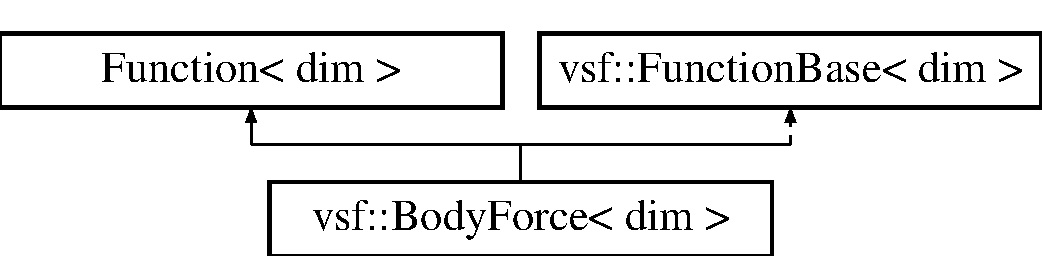
\includegraphics[height=2.000000cm]{classvsf_1_1BodyForce}
\end{center}
\end{figure}
\subsection*{Public Member Functions}
\begin{DoxyCompactItemize}
\item 
\hyperlink{classvsf_1_1BodyForce_ab0e2afab887f5ed138e9505dfd7a5a48}{Body\-Force} ()
\item 
virtual double \hyperlink{classvsf_1_1BodyForce_a02c4d3175f362852168899720754b7c0}{value} (const Point$<$ dim $>$ \&p, const unsigned int component=0) const 
\item 
virtual void \hyperlink{classvsf_1_1BodyForce_a1c23b3aaa12b0f2006cbfc2a1502d2d0}{value\-\_\-list} (const std\-::vector$<$ Point$<$ dim $>$ $>$ \&points, std\-::vector$<$ double $>$ \&values, const unsigned int component=0) const 
\end{DoxyCompactItemize}
\subsection*{Additional Inherited Members}


\subsection{Detailed Description}
\subsubsection*{template$<$int dim$>$class vsf\-::\-Body\-Force$<$ dim $>$}

The template class \hyperlink{classvsf_1_1BodyForce}{Body\-Force} gives the value of body force (on the right hand side of the elastic equation) in the requested point/s 

\subsection{Constructor \& Destructor Documentation}
\hypertarget{classvsf_1_1BodyForce_ab0e2afab887f5ed138e9505dfd7a5a48}{\index{vsf\-::\-Body\-Force@{vsf\-::\-Body\-Force}!Body\-Force@{Body\-Force}}
\index{Body\-Force@{Body\-Force}!vsf::BodyForce@{vsf\-::\-Body\-Force}}
\subsubsection[{Body\-Force}]{\setlength{\rightskip}{0pt plus 5cm}template$<$int dim$>$ {\bf vsf\-::\-Body\-Force}$<$ dim $>$\-::{\bf Body\-Force} (
\begin{DoxyParamCaption}
{}
\end{DoxyParamCaption}
)\hspace{0.3cm}{\ttfamily [inline]}}}\label{classvsf_1_1BodyForce_ab0e2afab887f5ed138e9505dfd7a5a48}


\subsection{Member Function Documentation}
\hypertarget{classvsf_1_1BodyForce_a02c4d3175f362852168899720754b7c0}{\index{vsf\-::\-Body\-Force@{vsf\-::\-Body\-Force}!value@{value}}
\index{value@{value}!vsf::BodyForce@{vsf\-::\-Body\-Force}}
\subsubsection[{value}]{\setlength{\rightskip}{0pt plus 5cm}template$<$int dim$>$ double {\bf vsf\-::\-Body\-Force}$<$ dim $>$\-::value (
\begin{DoxyParamCaption}
\item[{const Point$<$ dim $>$ \&}]{p, }
\item[{const unsigned int}]{component = {\ttfamily 0}}
\end{DoxyParamCaption}
) const\hspace{0.3cm}{\ttfamily [virtual]}}}\label{classvsf_1_1BodyForce_a02c4d3175f362852168899720754b7c0}
Right\-Hand\-Side\-::value extracts the value in one point (\char`\"{}p\char`\"{}). In the current implementation we consider a zero body force. To use a spatially variable shear modulus modify this method accordingly. \hypertarget{classvsf_1_1BodyForce_a1c23b3aaa12b0f2006cbfc2a1502d2d0}{\index{vsf\-::\-Body\-Force@{vsf\-::\-Body\-Force}!value\-\_\-list@{value\-\_\-list}}
\index{value\-\_\-list@{value\-\_\-list}!vsf::BodyForce@{vsf\-::\-Body\-Force}}
\subsubsection[{value\-\_\-list}]{\setlength{\rightskip}{0pt plus 5cm}template$<$int dim$>$ void {\bf vsf\-::\-Body\-Force}$<$ dim $>$\-::value\-\_\-list (
\begin{DoxyParamCaption}
\item[{const std\-::vector$<$ Point$<$ dim $>$ $>$ \&}]{points, }
\item[{std\-::vector$<$ double $>$ \&}]{values, }
\item[{const unsigned int}]{component = {\ttfamily 0}}
\end{DoxyParamCaption}
) const\hspace{0.3cm}{\ttfamily [virtual]}}}\label{classvsf_1_1BodyForce_a1c23b3aaa12b0f2006cbfc2a1502d2d0}
\hyperlink{classvsf_1_1BodyForce_a1c23b3aaa12b0f2006cbfc2a1502d2d0}{Body\-Force\-::value\-\_\-list} allows to extract values for several points (\char`\"{}points\char`\"{}) at once and outputs them in a vector (\char`\"{}values\char`\"{}). 

The documentation for this class was generated from the following file\-:\begin{DoxyCompactItemize}
\item 
\hyperlink{VE__fault__elastic_8cc}{V\-E\-\_\-fault\-\_\-elastic.\-cc}\end{DoxyCompactItemize}

\hypertarget{classvsf_1_1Dirichlet__BC}{\section{vsf\-:\-:Dirichlet\-\_\-\-B\-C$<$ dim $>$ Class Template Reference}
\label{classvsf_1_1Dirichlet__BC}\index{vsf\-::\-Dirichlet\-\_\-\-B\-C$<$ dim $>$@{vsf\-::\-Dirichlet\-\_\-\-B\-C$<$ dim $>$}}
}
Inheritance diagram for vsf\-:\-:Dirichlet\-\_\-\-B\-C$<$ dim $>$\-:\begin{figure}[H]
\begin{center}
\leavevmode
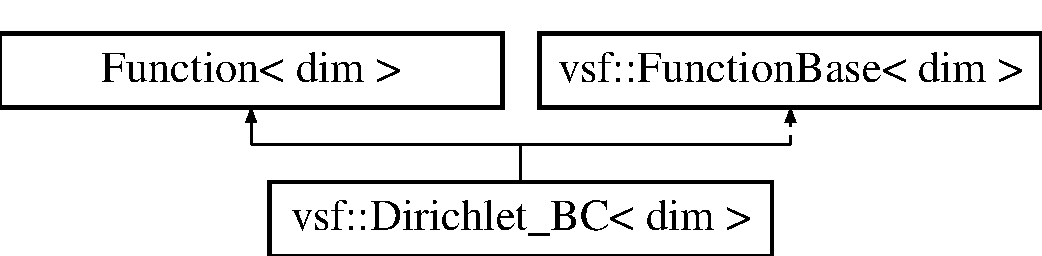
\includegraphics[height=2.000000cm]{classvsf_1_1Dirichlet__BC}
\end{center}
\end{figure}
\subsection*{Public Member Functions}
\begin{DoxyCompactItemize}
\item 
\hyperlink{classvsf_1_1Dirichlet__BC_a3fc7bb6aef647db39b9f1d4664b3740b}{Dirichlet\-\_\-\-B\-C} ()
\item 
virtual double \hyperlink{classvsf_1_1Dirichlet__BC_a9996ee81e6748568e3b069c12afdd674}{value} (const Point$<$ dim $>$ \&p, const unsigned int component=0) const 
\item 
virtual void \hyperlink{classvsf_1_1Dirichlet__BC_a883de335cd0c7709fba4b58d43a4dd4d}{value\-\_\-list} (const std\-::vector$<$ Point$<$ dim $>$ $>$ \&points, std\-::vector$<$ double $>$ \&values, const unsigned int component=0) const 
\end{DoxyCompactItemize}
\subsection*{Additional Inherited Members}


\subsection{Detailed Description}
\subsubsection*{template$<$int dim$>$class vsf\-::\-Dirichlet\-\_\-\-B\-C$<$ dim $>$}

The template class \hyperlink{classvsf_1_1Dirichlet__BC}{Dirichlet\-\_\-\-B\-C} computes the values of the non-\/homogeneous Dirichlet B\-C in each point. 

\subsection{Constructor \& Destructor Documentation}
\hypertarget{classvsf_1_1Dirichlet__BC_a3fc7bb6aef647db39b9f1d4664b3740b}{\index{vsf\-::\-Dirichlet\-\_\-\-B\-C@{vsf\-::\-Dirichlet\-\_\-\-B\-C}!Dirichlet\-\_\-\-B\-C@{Dirichlet\-\_\-\-B\-C}}
\index{Dirichlet\-\_\-\-B\-C@{Dirichlet\-\_\-\-B\-C}!vsf::Dirichlet_BC@{vsf\-::\-Dirichlet\-\_\-\-B\-C}}
\subsubsection[{Dirichlet\-\_\-\-B\-C}]{\setlength{\rightskip}{0pt plus 5cm}template$<$int dim$>$ {\bf vsf\-::\-Dirichlet\-\_\-\-B\-C}$<$ dim $>$\-::{\bf Dirichlet\-\_\-\-B\-C} (
\begin{DoxyParamCaption}
{}
\end{DoxyParamCaption}
)\hspace{0.3cm}{\ttfamily [inline]}}}\label{classvsf_1_1Dirichlet__BC_a3fc7bb6aef647db39b9f1d4664b3740b}


\subsection{Member Function Documentation}
\hypertarget{classvsf_1_1Dirichlet__BC_a9996ee81e6748568e3b069c12afdd674}{\index{vsf\-::\-Dirichlet\-\_\-\-B\-C@{vsf\-::\-Dirichlet\-\_\-\-B\-C}!value@{value}}
\index{value@{value}!vsf::Dirichlet_BC@{vsf\-::\-Dirichlet\-\_\-\-B\-C}}
\subsubsection[{value}]{\setlength{\rightskip}{0pt plus 5cm}template$<$int dim$>$ double {\bf vsf\-::\-Dirichlet\-\_\-\-B\-C}$<$ dim $>$\-::value (
\begin{DoxyParamCaption}
\item[{const Point$<$ dim $>$ \&}]{p, }
\item[{const unsigned int}]{component = {\ttfamily 0}}
\end{DoxyParamCaption}
) const\hspace{0.3cm}{\ttfamily [virtual]}}}\label{classvsf_1_1Dirichlet__BC_a9996ee81e6748568e3b069c12afdd674}
\hyperlink{classvsf_1_1Dirichlet__BC_a9996ee81e6748568e3b069c12afdd674}{Dirichlet\-\_\-\-B\-C\-::value} extracts the value in one point (\char`\"{}p\char`\"{}). To use a spatially variable B\-C modify this method accordingly. The displacement imposed at the boundary is only half the total displacement because we are only modeling half the domain.\hypertarget{classvsf_1_1Dirichlet__BC_a883de335cd0c7709fba4b58d43a4dd4d}{\index{vsf\-::\-Dirichlet\-\_\-\-B\-C@{vsf\-::\-Dirichlet\-\_\-\-B\-C}!value\-\_\-list@{value\-\_\-list}}
\index{value\-\_\-list@{value\-\_\-list}!vsf::Dirichlet_BC@{vsf\-::\-Dirichlet\-\_\-\-B\-C}}
\subsubsection[{value\-\_\-list}]{\setlength{\rightskip}{0pt plus 5cm}template$<$int dim$>$ void {\bf vsf\-::\-Dirichlet\-\_\-\-B\-C}$<$ dim $>$\-::value\-\_\-list (
\begin{DoxyParamCaption}
\item[{const std\-::vector$<$ Point$<$ dim $>$ $>$ \&}]{points, }
\item[{std\-::vector$<$ double $>$ \&}]{values, }
\item[{const unsigned int}]{component = {\ttfamily 0}}
\end{DoxyParamCaption}
) const\hspace{0.3cm}{\ttfamily [virtual]}}}\label{classvsf_1_1Dirichlet__BC_a883de335cd0c7709fba4b58d43a4dd4d}
\hyperlink{classvsf_1_1Dirichlet__BC_a883de335cd0c7709fba4b58d43a4dd4d}{Dirichlet\-\_\-\-B\-C\-::value\-\_\-list} allows to extract values for several points (\char`\"{}points\char`\"{}) at once and outputs them in a vector (\char`\"{}values\char`\"{}). 

The documentation for this class was generated from the following file\-:\begin{DoxyCompactItemize}
\item 
\hyperlink{VE__fault__elastic_8cc}{V\-E\-\_\-fault\-\_\-elastic.\-cc}\end{DoxyCompactItemize}

\hypertarget{classvsf_1_1FunctionBase}{\section{vsf\-:\-:Function\-Base$<$ dim $>$ Class Template Reference}
\label{classvsf_1_1FunctionBase}\index{vsf\-::\-Function\-Base$<$ dim $>$@{vsf\-::\-Function\-Base$<$ dim $>$}}
}
Inheritance diagram for vsf\-:\-:Function\-Base$<$ dim $>$\-:\begin{figure}[H]
\begin{center}
\leavevmode
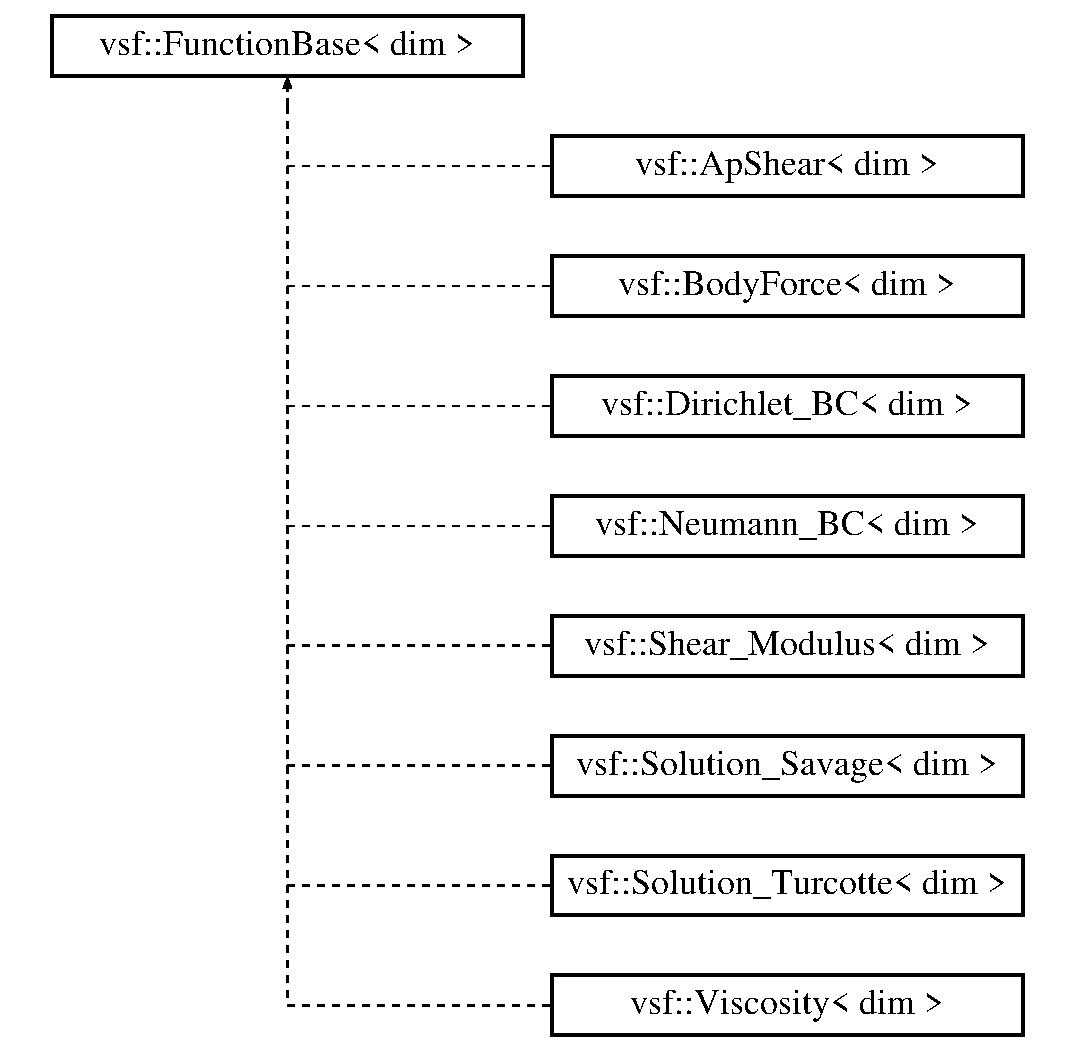
\includegraphics[height=9.000000cm]{classvsf_1_1FunctionBase}
\end{center}
\end{figure}
\subsection*{Static Protected Attributes}
\begin{DoxyCompactItemize}
\item 
static const double \hyperlink{classvsf_1_1FunctionBase_ad2bf6791357d301b7d838b6188ef646e}{width} = 2.\-0e5
\item 
static const double \hyperlink{classvsf_1_1FunctionBase_acfffb54eadb79217d150a73e3797b25a}{height} = 1.\-0e5
\item 
static const double \hyperlink{classvsf_1_1FunctionBase_ae06ffa81ca26e9ead535d50596d852c1}{locked\-\_\-depth} = 0.\-25e5
\item 
static const double \hyperlink{classvsf_1_1FunctionBase_a70a9a9f8a1a73386e582c529338f2d5e}{boundary\-\_\-displacement} = 10
\item 
static const double \hyperlink{classvsf_1_1FunctionBase_a342cfaf03d11de71ca34234f48e8825e}{boundary\-\_\-stress} = 1e5
\item 
static const double \hyperlink{classvsf_1_1FunctionBase_a6fc26a27ba1d3a74dfe144a16d7893aa}{shear\-\_\-modulus} = 1.\-0e11
\item 
static const double \hyperlink{classvsf_1_1FunctionBase_af8a2b8711f526a821e1a37a396c9b48f}{viscosity} = 1e20
\end{DoxyCompactItemize}


\subsection{Detailed Description}
\subsubsection*{template$<$int dim$>$class vsf\-::\-Function\-Base$<$ dim $>$}

We declare and define some function classes that represent the body force, the viscosity and the boundary values. For simplicity we have chosen to define all relevant parameters in a base class, which later will serve as the base class for the rest of the classes. These parameters are the width and height of the model (\hyperlink{classvsf_1_1FunctionBase_ad2bf6791357d301b7d838b6188ef646e}{Function\-Base\-::width} and \hyperlink{classvsf_1_1FunctionBase_acfffb54eadb79217d150a73e3797b25a}{Function\-Base\-::height}), lock depth $d$ (\hyperlink{classvsf_1_1FunctionBase_ae06ffa81ca26e9ead535d50596d852c1}{Function\-Base\-::locked\-\_\-depth}), the imposed displacement at the boundary $U$ (\hyperlink{classvsf_1_1FunctionBase_a70a9a9f8a1a73386e582c529338f2d5e}{Function\-Base\-::boundary\-\_\-displacement}) and the imposed stress at the boundary $S$ (\hyperlink{classvsf_1_1FunctionBase_a342cfaf03d11de71ca34234f48e8825e}{Function\-Base\-::boundary\-\_\-stress}).

\begin{DoxyNote}{Note}
These parameters have to be hardcoded here because the solution and boundary conditions classes are derived from \href{https://www.dealii.org/8.2.0/doxygen/deal.II/classFunction.html}{\tt Function} and are used directly by other deal.\-I\-I class functions. Adding any extra input parameters in a class that inherits from \href{https://www.dealii.org/8.2.0/doxygen/deal.II/classFunction.html}{\tt Function} would require modifying the source code. Another option would be to input these parameter via an input file (see deal.\-I\-I tutorial \href{https://www.dealii.org/8.2.0/doxygen/deal.II/step_33.html}{\tt step-\/33}).
\end{DoxyNote}
All the parameters used in the code are set here to keep things in order. 

\subsection{Member Data Documentation}
\hypertarget{classvsf_1_1FunctionBase_a70a9a9f8a1a73386e582c529338f2d5e}{\index{vsf\-::\-Function\-Base@{vsf\-::\-Function\-Base}!boundary\-\_\-displacement@{boundary\-\_\-displacement}}
\index{boundary\-\_\-displacement@{boundary\-\_\-displacement}!vsf::FunctionBase@{vsf\-::\-Function\-Base}}
\subsubsection[{boundary\-\_\-displacement}]{\setlength{\rightskip}{0pt plus 5cm}template$<$int dim$>$ const double {\bf vsf\-::\-Function\-Base}$<$ dim $>$\-::boundary\-\_\-displacement = 10\hspace{0.3cm}{\ttfamily [static]}, {\ttfamily [protected]}}}\label{classvsf_1_1FunctionBase_a70a9a9f8a1a73386e582c529338f2d5e}
Displacement imposed in some boundaries. \hypertarget{classvsf_1_1FunctionBase_a342cfaf03d11de71ca34234f48e8825e}{\index{vsf\-::\-Function\-Base@{vsf\-::\-Function\-Base}!boundary\-\_\-stress@{boundary\-\_\-stress}}
\index{boundary\-\_\-stress@{boundary\-\_\-stress}!vsf::FunctionBase@{vsf\-::\-Function\-Base}}
\subsubsection[{boundary\-\_\-stress}]{\setlength{\rightskip}{0pt plus 5cm}template$<$int dim$>$ const double {\bf vsf\-::\-Function\-Base}$<$ dim $>$\-::boundary\-\_\-stress = 1e5\hspace{0.3cm}{\ttfamily [static]}, {\ttfamily [protected]}}}\label{classvsf_1_1FunctionBase_a342cfaf03d11de71ca34234f48e8825e}
Stress imposed in some boundaries. \hypertarget{classvsf_1_1FunctionBase_acfffb54eadb79217d150a73e3797b25a}{\index{vsf\-::\-Function\-Base@{vsf\-::\-Function\-Base}!height@{height}}
\index{height@{height}!vsf::FunctionBase@{vsf\-::\-Function\-Base}}
\subsubsection[{height}]{\setlength{\rightskip}{0pt plus 5cm}template$<$int dim$>$ const double {\bf vsf\-::\-Function\-Base}$<$ dim $>$\-::height = 1.\-0e5\hspace{0.3cm}{\ttfamily [static]}, {\ttfamily [protected]}}}\label{classvsf_1_1FunctionBase_acfffb54eadb79217d150a73e3797b25a}
Model's height. \hypertarget{classvsf_1_1FunctionBase_ae06ffa81ca26e9ead535d50596d852c1}{\index{vsf\-::\-Function\-Base@{vsf\-::\-Function\-Base}!locked\-\_\-depth@{locked\-\_\-depth}}
\index{locked\-\_\-depth@{locked\-\_\-depth}!vsf::FunctionBase@{vsf\-::\-Function\-Base}}
\subsubsection[{locked\-\_\-depth}]{\setlength{\rightskip}{0pt plus 5cm}template$<$int dim$>$ const double {\bf vsf\-::\-Function\-Base}$<$ dim $>$\-::locked\-\_\-depth = 0.\-25e5\hspace{0.3cm}{\ttfamily [static]}, {\ttfamily [protected]}}}\label{classvsf_1_1FunctionBase_ae06ffa81ca26e9ead535d50596d852c1}
Depth of the locked region. \hypertarget{classvsf_1_1FunctionBase_a6fc26a27ba1d3a74dfe144a16d7893aa}{\index{vsf\-::\-Function\-Base@{vsf\-::\-Function\-Base}!shear\-\_\-modulus@{shear\-\_\-modulus}}
\index{shear\-\_\-modulus@{shear\-\_\-modulus}!vsf::FunctionBase@{vsf\-::\-Function\-Base}}
\subsubsection[{shear\-\_\-modulus}]{\setlength{\rightskip}{0pt plus 5cm}template$<$int dim$>$ const double {\bf vsf\-::\-Function\-Base}$<$ dim $>$\-::shear\-\_\-modulus = 1.\-0e11\hspace{0.3cm}{\ttfamily [static]}, {\ttfamily [protected]}}}\label{classvsf_1_1FunctionBase_a6fc26a27ba1d3a74dfe144a16d7893aa}
Reference shear modulus. \hypertarget{classvsf_1_1FunctionBase_af8a2b8711f526a821e1a37a396c9b48f}{\index{vsf\-::\-Function\-Base@{vsf\-::\-Function\-Base}!viscosity@{viscosity}}
\index{viscosity@{viscosity}!vsf::FunctionBase@{vsf\-::\-Function\-Base}}
\subsubsection[{viscosity}]{\setlength{\rightskip}{0pt plus 5cm}template$<$int dim$>$ const double {\bf vsf\-::\-Function\-Base}$<$ dim $>$\-::viscosity = 1e20\hspace{0.3cm}{\ttfamily [static]}, {\ttfamily [protected]}}}\label{classvsf_1_1FunctionBase_af8a2b8711f526a821e1a37a396c9b48f}
Reference viscosity. \hypertarget{classvsf_1_1FunctionBase_ad2bf6791357d301b7d838b6188ef646e}{\index{vsf\-::\-Function\-Base@{vsf\-::\-Function\-Base}!width@{width}}
\index{width@{width}!vsf::FunctionBase@{vsf\-::\-Function\-Base}}
\subsubsection[{width}]{\setlength{\rightskip}{0pt plus 5cm}template$<$int dim$>$ const double {\bf vsf\-::\-Function\-Base}$<$ dim $>$\-::width = 2.\-0e5\hspace{0.3cm}{\ttfamily [static]}, {\ttfamily [protected]}}}\label{classvsf_1_1FunctionBase_ad2bf6791357d301b7d838b6188ef646e}
Model's width. Will not be used here, but we want to keep input parameters together. 

The documentation for this class was generated from the following file\-:\begin{DoxyCompactItemize}
\item 
\hyperlink{VE__fault__elastic_8cc}{V\-E\-\_\-fault\-\_\-elastic.\-cc}\end{DoxyCompactItemize}

\hypertarget{classvsf_1_1Neumann__BC}{\section{vsf\-:\-:Neumann\-\_\-\-B\-C$<$ dim $>$ Class Template Reference}
\label{classvsf_1_1Neumann__BC}\index{vsf\-::\-Neumann\-\_\-\-B\-C$<$ dim $>$@{vsf\-::\-Neumann\-\_\-\-B\-C$<$ dim $>$}}
}
Inheritance diagram for vsf\-:\-:Neumann\-\_\-\-B\-C$<$ dim $>$\-:\begin{figure}[H]
\begin{center}
\leavevmode
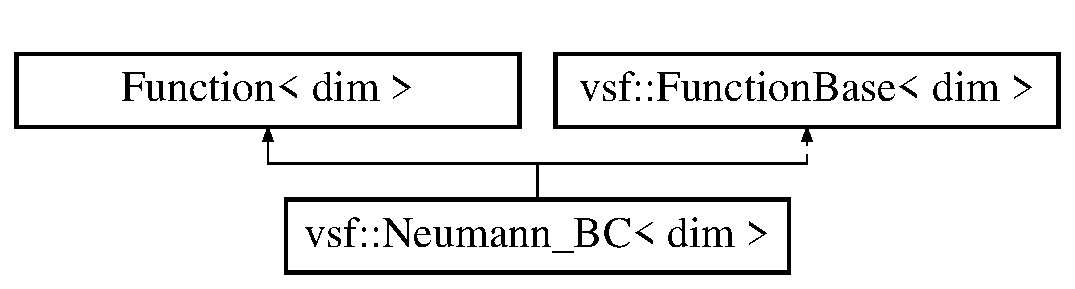
\includegraphics[height=2.000000cm]{classvsf_1_1Neumann__BC}
\end{center}
\end{figure}
\subsection*{Public Member Functions}
\begin{DoxyCompactItemize}
\item 
\hyperlink{classvsf_1_1Neumann__BC_a8b36c26330ec21aa09f6887f1a49a329}{Neumann\-\_\-\-B\-C} ()
\item 
virtual double \hyperlink{classvsf_1_1Neumann__BC_addccdf65c1e5367b004289db3b0b96a5}{value} (const Point$<$ dim $>$ \&p, const unsigned int component=0) const 
\item 
virtual void \hyperlink{classvsf_1_1Neumann__BC_a2e1fe62899a58c70bbb4e9021858427e}{value\-\_\-list} (const std\-::vector$<$ Point$<$ dim $>$ $>$ \&points, std\-::vector$<$ double $>$ \&values, const unsigned int component=0) const 
\end{DoxyCompactItemize}
\subsection*{Additional Inherited Members}


\subsection{Detailed Description}
\subsubsection*{template$<$int dim$>$class vsf\-::\-Neumann\-\_\-\-B\-C$<$ dim $>$}

The template class \hyperlink{classvsf_1_1Neumann__BC}{Neumann\-\_\-\-B\-C} computes the values of the non-\/homogeneous B\-C in each point. 

\subsection{Constructor \& Destructor Documentation}
\hypertarget{classvsf_1_1Neumann__BC_a8b36c26330ec21aa09f6887f1a49a329}{\index{vsf\-::\-Neumann\-\_\-\-B\-C@{vsf\-::\-Neumann\-\_\-\-B\-C}!Neumann\-\_\-\-B\-C@{Neumann\-\_\-\-B\-C}}
\index{Neumann\-\_\-\-B\-C@{Neumann\-\_\-\-B\-C}!vsf::Neumann_BC@{vsf\-::\-Neumann\-\_\-\-B\-C}}
\subsubsection[{Neumann\-\_\-\-B\-C}]{\setlength{\rightskip}{0pt plus 5cm}template$<$int dim$>$ {\bf vsf\-::\-Neumann\-\_\-\-B\-C}$<$ dim $>$\-::{\bf Neumann\-\_\-\-B\-C} (
\begin{DoxyParamCaption}
{}
\end{DoxyParamCaption}
)\hspace{0.3cm}{\ttfamily [inline]}}}\label{classvsf_1_1Neumann__BC_a8b36c26330ec21aa09f6887f1a49a329}


\subsection{Member Function Documentation}
\hypertarget{classvsf_1_1Neumann__BC_addccdf65c1e5367b004289db3b0b96a5}{\index{vsf\-::\-Neumann\-\_\-\-B\-C@{vsf\-::\-Neumann\-\_\-\-B\-C}!value@{value}}
\index{value@{value}!vsf::Neumann_BC@{vsf\-::\-Neumann\-\_\-\-B\-C}}
\subsubsection[{value}]{\setlength{\rightskip}{0pt plus 5cm}template$<$int dim$>$ double {\bf vsf\-::\-Neumann\-\_\-\-B\-C}$<$ dim $>$\-::value (
\begin{DoxyParamCaption}
\item[{const Point$<$ dim $>$ \&}]{p, }
\item[{const unsigned int}]{component = {\ttfamily 0}}
\end{DoxyParamCaption}
) const\hspace{0.3cm}{\ttfamily [virtual]}}}\label{classvsf_1_1Neumann__BC_addccdf65c1e5367b004289db3b0b96a5}
\hyperlink{classvsf_1_1Neumann__BC_addccdf65c1e5367b004289db3b0b96a5}{Neumann\-\_\-\-B\-C\-::value} extracts the value in one point (\char`\"{}p\char`\"{}). To use a spatially variable B\-C modify this method accordingly. \hypertarget{classvsf_1_1Neumann__BC_a2e1fe62899a58c70bbb4e9021858427e}{\index{vsf\-::\-Neumann\-\_\-\-B\-C@{vsf\-::\-Neumann\-\_\-\-B\-C}!value\-\_\-list@{value\-\_\-list}}
\index{value\-\_\-list@{value\-\_\-list}!vsf::Neumann_BC@{vsf\-::\-Neumann\-\_\-\-B\-C}}
\subsubsection[{value\-\_\-list}]{\setlength{\rightskip}{0pt plus 5cm}template$<$int dim$>$ void {\bf vsf\-::\-Neumann\-\_\-\-B\-C}$<$ dim $>$\-::value\-\_\-list (
\begin{DoxyParamCaption}
\item[{const std\-::vector$<$ Point$<$ dim $>$ $>$ \&}]{points, }
\item[{std\-::vector$<$ double $>$ \&}]{values, }
\item[{const unsigned int}]{component = {\ttfamily 0}}
\end{DoxyParamCaption}
) const\hspace{0.3cm}{\ttfamily [virtual]}}}\label{classvsf_1_1Neumann__BC_a2e1fe62899a58c70bbb4e9021858427e}
\hyperlink{classvsf_1_1Neumann__BC_a2e1fe62899a58c70bbb4e9021858427e}{Neumann\-\_\-\-B\-C\-::value\-\_\-list} allows to extract values for several points (\char`\"{}points\char`\"{}) at once and outputs them in a vector (\char`\"{}values\char`\"{}). 

The documentation for this class was generated from the following file\-:\begin{DoxyCompactItemize}
\item 
\hyperlink{VE__fault__elastic_8cc}{V\-E\-\_\-fault\-\_\-elastic.\-cc}\end{DoxyCompactItemize}

\hypertarget{structvsf_1_1PointHistory}{\section{vsf\-:\-:Point\-History$<$ dim $>$ Struct Template Reference}
\label{structvsf_1_1PointHistory}\index{vsf\-::\-Point\-History$<$ dim $>$@{vsf\-::\-Point\-History$<$ dim $>$}}
}
\subsection*{Public Attributes}
\begin{DoxyCompactItemize}
\item 
Tensor$<$ 1, 2 $>$ \hyperlink{structvsf_1_1PointHistory_a24aabd1a3f1b17bbd0a69d5f630037d2}{new\-\_\-v\-\_\-strain}
\end{DoxyCompactItemize}


\subsection{Detailed Description}
\subsubsection*{template$<$int dim$>$struct vsf\-::\-Point\-History$<$ dim $>$}

We first define a structure where we will store the old data that we will need to compute the right hand side of the equation. In this case it is enough if we save the viscous strain from the previous time step. 

\subsection{Member Data Documentation}
\hypertarget{structvsf_1_1PointHistory_a24aabd1a3f1b17bbd0a69d5f630037d2}{\index{vsf\-::\-Point\-History@{vsf\-::\-Point\-History}!new\-\_\-v\-\_\-strain@{new\-\_\-v\-\_\-strain}}
\index{new\-\_\-v\-\_\-strain@{new\-\_\-v\-\_\-strain}!vsf::PointHistory@{vsf\-::\-Point\-History}}
\subsubsection[{new\-\_\-v\-\_\-strain}]{\setlength{\rightskip}{0pt plus 5cm}template$<$int dim$>$ Tensor$<$1,2$>$ {\bf vsf\-::\-Point\-History}$<$ dim $>$\-::new\-\_\-v\-\_\-strain}}\label{structvsf_1_1PointHistory_a24aabd1a3f1b17bbd0a69d5f630037d2}


The documentation for this struct was generated from the following file\-:\begin{DoxyCompactItemize}
\item 
\hyperlink{VE__fault__elastic_8cc}{V\-E\-\_\-fault\-\_\-elastic.\-cc}\end{DoxyCompactItemize}

\hypertarget{classvsf_1_1Shear__Modulus}{\section{vsf\-:\-:Shear\-\_\-\-Modulus$<$ dim $>$ Class Template Reference}
\label{classvsf_1_1Shear__Modulus}\index{vsf\-::\-Shear\-\_\-\-Modulus$<$ dim $>$@{vsf\-::\-Shear\-\_\-\-Modulus$<$ dim $>$}}
}
Inheritance diagram for vsf\-:\-:Shear\-\_\-\-Modulus$<$ dim $>$\-:\begin{figure}[H]
\begin{center}
\leavevmode
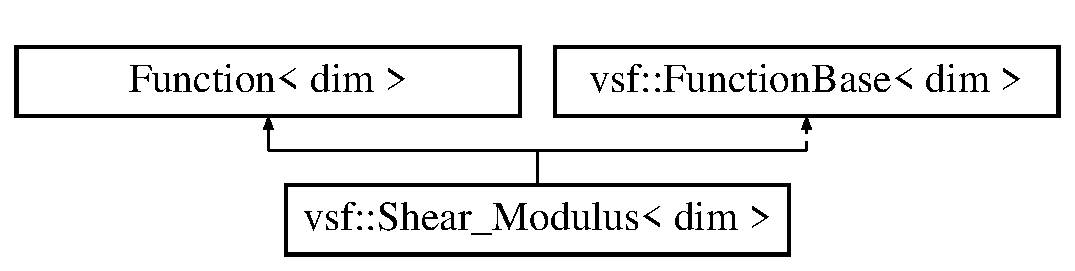
\includegraphics[height=2.000000cm]{classvsf_1_1Shear__Modulus}
\end{center}
\end{figure}
\subsection*{Public Member Functions}
\begin{DoxyCompactItemize}
\item 
\hyperlink{classvsf_1_1Shear__Modulus_a00275a013eac84ac1cce403d183f2488}{Shear\-\_\-\-Modulus} ()
\item 
virtual double \hyperlink{classvsf_1_1Shear__Modulus_a914f7afda36d3cfa6e80563f8b7444cc}{value} (const Point$<$ dim $>$ \&p, const unsigned int component=0) const 
\item 
virtual void \hyperlink{classvsf_1_1Shear__Modulus_a01a61b73422dbb0819ac993b97739afb}{value\-\_\-list} (const std\-::vector$<$ Point$<$ dim $>$ $>$ \&points, std\-::vector$<$ double $>$ \&values, const unsigned int component=0) const 
\end{DoxyCompactItemize}
\subsection*{Additional Inherited Members}


\subsection{Detailed Description}
\subsubsection*{template$<$int dim$>$class vsf\-::\-Shear\-\_\-\-Modulus$<$ dim $>$}

The template class \hyperlink{classvsf_1_1Shear__Modulus}{Shear\-\_\-\-Modulus} gives the value of the shear modulus in the requested point/s 

\subsection{Constructor \& Destructor Documentation}
\hypertarget{classvsf_1_1Shear__Modulus_a00275a013eac84ac1cce403d183f2488}{\index{vsf\-::\-Shear\-\_\-\-Modulus@{vsf\-::\-Shear\-\_\-\-Modulus}!Shear\-\_\-\-Modulus@{Shear\-\_\-\-Modulus}}
\index{Shear\-\_\-\-Modulus@{Shear\-\_\-\-Modulus}!vsf::Shear_Modulus@{vsf\-::\-Shear\-\_\-\-Modulus}}
\subsubsection[{Shear\-\_\-\-Modulus}]{\setlength{\rightskip}{0pt plus 5cm}template$<$int dim$>$ {\bf vsf\-::\-Shear\-\_\-\-Modulus}$<$ dim $>$\-::{\bf Shear\-\_\-\-Modulus} (
\begin{DoxyParamCaption}
{}
\end{DoxyParamCaption}
)\hspace{0.3cm}{\ttfamily [inline]}}}\label{classvsf_1_1Shear__Modulus_a00275a013eac84ac1cce403d183f2488}


\subsection{Member Function Documentation}
\hypertarget{classvsf_1_1Shear__Modulus_a914f7afda36d3cfa6e80563f8b7444cc}{\index{vsf\-::\-Shear\-\_\-\-Modulus@{vsf\-::\-Shear\-\_\-\-Modulus}!value@{value}}
\index{value@{value}!vsf::Shear_Modulus@{vsf\-::\-Shear\-\_\-\-Modulus}}
\subsubsection[{value}]{\setlength{\rightskip}{0pt plus 5cm}template$<$int dim$>$ double {\bf vsf\-::\-Shear\-\_\-\-Modulus}$<$ dim $>$\-::value (
\begin{DoxyParamCaption}
\item[{const Point$<$ dim $>$ \&}]{p, }
\item[{const unsigned int}]{component = {\ttfamily 0}}
\end{DoxyParamCaption}
) const\hspace{0.3cm}{\ttfamily [virtual]}}}\label{classvsf_1_1Shear__Modulus_a914f7afda36d3cfa6e80563f8b7444cc}
\hyperlink{classvsf_1_1Shear__Modulus_a914f7afda36d3cfa6e80563f8b7444cc}{Shear\-\_\-\-Modulus\-::value} extracts the value in one point (\char`\"{}p\char`\"{}). In the current implementation we consider a uniform shear modulus. To use a spatially variable shear modulus modify this method accordingly. \hypertarget{classvsf_1_1Shear__Modulus_a01a61b73422dbb0819ac993b97739afb}{\index{vsf\-::\-Shear\-\_\-\-Modulus@{vsf\-::\-Shear\-\_\-\-Modulus}!value\-\_\-list@{value\-\_\-list}}
\index{value\-\_\-list@{value\-\_\-list}!vsf::Shear_Modulus@{vsf\-::\-Shear\-\_\-\-Modulus}}
\subsubsection[{value\-\_\-list}]{\setlength{\rightskip}{0pt plus 5cm}template$<$int dim$>$ void {\bf vsf\-::\-Shear\-\_\-\-Modulus}$<$ dim $>$\-::value\-\_\-list (
\begin{DoxyParamCaption}
\item[{const std\-::vector$<$ Point$<$ dim $>$ $>$ \&}]{points, }
\item[{std\-::vector$<$ double $>$ \&}]{values, }
\item[{const unsigned int}]{component = {\ttfamily 0}}
\end{DoxyParamCaption}
) const\hspace{0.3cm}{\ttfamily [virtual]}}}\label{classvsf_1_1Shear__Modulus_a01a61b73422dbb0819ac993b97739afb}
\hyperlink{classvsf_1_1Shear__Modulus_a01a61b73422dbb0819ac993b97739afb}{Shear\-\_\-\-Modulus\-::value\-\_\-list} allows to extract values for several points (\char`\"{}points\char`\"{}) at once and outputs them in a vector (\char`\"{}values\char`\"{}). 

The documentation for this class was generated from the following file\-:\begin{DoxyCompactItemize}
\item 
\hyperlink{VE__fault__elastic_8cc}{V\-E\-\_\-fault\-\_\-elastic.\-cc}\end{DoxyCompactItemize}

\hypertarget{classvsf_1_1Solution__Savage}{\section{vsf\-:\-:Solution\-\_\-\-Savage$<$ dim $>$ Class Template Reference}
\label{classvsf_1_1Solution__Savage}\index{vsf\-::\-Solution\-\_\-\-Savage$<$ dim $>$@{vsf\-::\-Solution\-\_\-\-Savage$<$ dim $>$}}
}
Inheritance diagram for vsf\-:\-:Solution\-\_\-\-Savage$<$ dim $>$\-:\begin{figure}[H]
\begin{center}
\leavevmode
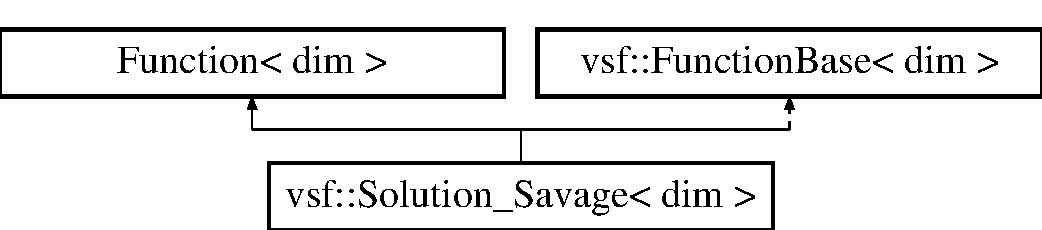
\includegraphics[height=2.000000cm]{classvsf_1_1Solution__Savage}
\end{center}
\end{figure}
\subsection*{Public Member Functions}
\begin{DoxyCompactItemize}
\item 
\hyperlink{classvsf_1_1Solution__Savage_a3cb39f3c76ce35ecaf75c83a9f8ec396}{Solution\-\_\-\-Savage} ()
\item 
virtual double \hyperlink{classvsf_1_1Solution__Savage_a7cc24cd1892ce82f00e0c8c02700897d}{value} (const Point$<$ dim $>$ \&p, const unsigned int component=0) const 
\item 
virtual void \hyperlink{classvsf_1_1Solution__Savage_a7dd79bf997cb39e1916fb0e28e8a7161}{value\-\_\-list} (const std\-::vector$<$ Point$<$ dim $>$ $>$ \&points, std\-::vector$<$ double $>$ \&values, const unsigned int component=0) const 
\end{DoxyCompactItemize}
\subsection*{Additional Inherited Members}


\subsection{Detailed Description}
\subsubsection*{template$<$int dim$>$class vsf\-::\-Solution\-\_\-\-Savage$<$ dim $>$}

This class is used to compute the analytical solution of the surface displacement caused by a fault in a completely elastic medium using \cite{savage_burford_73}. 

\subsection{Constructor \& Destructor Documentation}
\hypertarget{classvsf_1_1Solution__Savage_a3cb39f3c76ce35ecaf75c83a9f8ec396}{\index{vsf\-::\-Solution\-\_\-\-Savage@{vsf\-::\-Solution\-\_\-\-Savage}!Solution\-\_\-\-Savage@{Solution\-\_\-\-Savage}}
\index{Solution\-\_\-\-Savage@{Solution\-\_\-\-Savage}!vsf::Solution_Savage@{vsf\-::\-Solution\-\_\-\-Savage}}
\subsubsection[{Solution\-\_\-\-Savage}]{\setlength{\rightskip}{0pt plus 5cm}template$<$int dim$>$ {\bf vsf\-::\-Solution\-\_\-\-Savage}$<$ dim $>$\-::{\bf Solution\-\_\-\-Savage} (
\begin{DoxyParamCaption}
{}
\end{DoxyParamCaption}
)\hspace{0.3cm}{\ttfamily [inline]}}}\label{classvsf_1_1Solution__Savage_a3cb39f3c76ce35ecaf75c83a9f8ec396}


\subsection{Member Function Documentation}
\hypertarget{classvsf_1_1Solution__Savage_a7cc24cd1892ce82f00e0c8c02700897d}{\index{vsf\-::\-Solution\-\_\-\-Savage@{vsf\-::\-Solution\-\_\-\-Savage}!value@{value}}
\index{value@{value}!vsf::Solution_Savage@{vsf\-::\-Solution\-\_\-\-Savage}}
\subsubsection[{value}]{\setlength{\rightskip}{0pt plus 5cm}template$<$int dim$>$ double {\bf vsf\-::\-Solution\-\_\-\-Savage}$<$ dim $>$\-::value (
\begin{DoxyParamCaption}
\item[{const Point$<$ dim $>$ \&}]{p, }
\item[{const unsigned int}]{component = {\ttfamily 0}}
\end{DoxyParamCaption}
) const\hspace{0.3cm}{\ttfamily [virtual]}}}\label{classvsf_1_1Solution__Savage_a7cc24cd1892ce82f00e0c8c02700897d}
\hyperlink{classvsf_1_1Solution__Savage_a7cc24cd1892ce82f00e0c8c02700897d}{Solution\-\_\-\-Savage\-::value} extracts the value of the analytical solution in one point (\char`\"{}p\char`\"{}). This solution is only valid at the surface, therefore, if the point at which it will be evaluated is not in the surface, an exception will be thrown.\hypertarget{classvsf_1_1Solution__Savage_a7dd79bf997cb39e1916fb0e28e8a7161}{\index{vsf\-::\-Solution\-\_\-\-Savage@{vsf\-::\-Solution\-\_\-\-Savage}!value\-\_\-list@{value\-\_\-list}}
\index{value\-\_\-list@{value\-\_\-list}!vsf::Solution_Savage@{vsf\-::\-Solution\-\_\-\-Savage}}
\subsubsection[{value\-\_\-list}]{\setlength{\rightskip}{0pt plus 5cm}template$<$int dim$>$ void {\bf vsf\-::\-Solution\-\_\-\-Savage}$<$ dim $>$\-::value\-\_\-list (
\begin{DoxyParamCaption}
\item[{const std\-::vector$<$ Point$<$ dim $>$ $>$ \&}]{points, }
\item[{std\-::vector$<$ double $>$ \&}]{values, }
\item[{const unsigned int}]{component = {\ttfamily 0}}
\end{DoxyParamCaption}
) const\hspace{0.3cm}{\ttfamily [virtual]}}}\label{classvsf_1_1Solution__Savage_a7dd79bf997cb39e1916fb0e28e8a7161}
\hyperlink{classvsf_1_1Solution__Savage_a7dd79bf997cb39e1916fb0e28e8a7161}{Solution\-\_\-\-Savage\-::value\-\_\-list} allows to extract values for several points (\char`\"{}points\char`\"{}) at once and outputs them in a vector (\char`\"{}values\char`\"{}). 

The documentation for this class was generated from the following file\-:\begin{DoxyCompactItemize}
\item 
\hyperlink{VE__fault__elastic_8cc}{V\-E\-\_\-fault\-\_\-elastic.\-cc}\end{DoxyCompactItemize}

\hypertarget{classvsf_1_1Solution__Turcotte}{\section{vsf\-:\-:Solution\-\_\-\-Turcotte$<$ dim $>$ Class Template Reference}
\label{classvsf_1_1Solution__Turcotte}\index{vsf\-::\-Solution\-\_\-\-Turcotte$<$ dim $>$@{vsf\-::\-Solution\-\_\-\-Turcotte$<$ dim $>$}}
}
Inheritance diagram for vsf\-:\-:Solution\-\_\-\-Turcotte$<$ dim $>$\-:\begin{figure}[H]
\begin{center}
\leavevmode
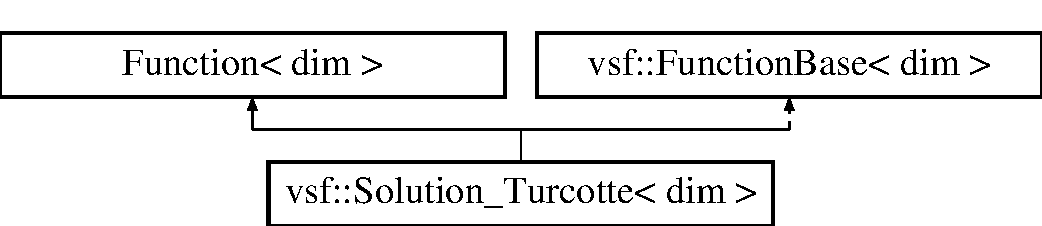
\includegraphics[height=2.000000cm]{classvsf_1_1Solution__Turcotte}
\end{center}
\end{figure}
\subsection*{Public Member Functions}
\begin{DoxyCompactItemize}
\item 
\hyperlink{classvsf_1_1Solution__Turcotte_a30c7ada8fc223741d07f3e4f5f15f6be}{Solution\-\_\-\-Turcotte} ()
\item 
virtual double \hyperlink{classvsf_1_1Solution__Turcotte_a14a3516d1011ab7cb0bbc9e95ba281f2}{value} (const Point$<$ dim $>$ \&p, const unsigned int component=0) const 
\item 
virtual void \hyperlink{classvsf_1_1Solution__Turcotte_a1208e498d2ce30b41a47ebe2d8c8c058}{value\-\_\-list} (const std\-::vector$<$ Point$<$ dim $>$ $>$ \&points, std\-::vector$<$ double $>$ \&values, const unsigned int component=0) const 
\item 
virtual void \hyperlink{classvsf_1_1Solution__Turcotte_af641b6a8b3a9685773e61736160a5fb2}{get\-\_\-time} (const double \&t)
\end{DoxyCompactItemize}
\subsection*{Private Attributes}
\begin{DoxyCompactItemize}
\item 
double \hyperlink{classvsf_1_1Solution__Turcotte_a5f58ba10fac1adc353f0e4889f9037b6}{time}
\end{DoxyCompactItemize}
\subsection*{Additional Inherited Members}


\subsection{Detailed Description}
\subsubsection*{template$<$int dim$>$class vsf\-::\-Solution\-\_\-\-Turcotte$<$ dim $>$}

This class is used to compute the analytical solution of the surface displacement caused by a fault in a completely elastic medium. we use Turcotte and Spence viscouse model\cite{turcotte_spence_74}. and applyt the correspondence principle to obtain the viscoelastic solution. 

\subsection{Constructor \& Destructor Documentation}
\hypertarget{classvsf_1_1Solution__Turcotte_a30c7ada8fc223741d07f3e4f5f15f6be}{\index{vsf\-::\-Solution\-\_\-\-Turcotte@{vsf\-::\-Solution\-\_\-\-Turcotte}!Solution\-\_\-\-Turcotte@{Solution\-\_\-\-Turcotte}}
\index{Solution\-\_\-\-Turcotte@{Solution\-\_\-\-Turcotte}!vsf::Solution_Turcotte@{vsf\-::\-Solution\-\_\-\-Turcotte}}
\subsubsection[{Solution\-\_\-\-Turcotte}]{\setlength{\rightskip}{0pt plus 5cm}template$<$int dim$>$ {\bf vsf\-::\-Solution\-\_\-\-Turcotte}$<$ dim $>$\-::{\bf Solution\-\_\-\-Turcotte} (
\begin{DoxyParamCaption}
{}
\end{DoxyParamCaption}
)\hspace{0.3cm}{\ttfamily [inline]}}}\label{classvsf_1_1Solution__Turcotte_a30c7ada8fc223741d07f3e4f5f15f6be}


\subsection{Member Function Documentation}
\hypertarget{classvsf_1_1Solution__Turcotte_af641b6a8b3a9685773e61736160a5fb2}{\index{vsf\-::\-Solution\-\_\-\-Turcotte@{vsf\-::\-Solution\-\_\-\-Turcotte}!get\-\_\-time@{get\-\_\-time}}
\index{get\-\_\-time@{get\-\_\-time}!vsf::Solution_Turcotte@{vsf\-::\-Solution\-\_\-\-Turcotte}}
\subsubsection[{get\-\_\-time}]{\setlength{\rightskip}{0pt plus 5cm}template$<$int dim$>$ void {\bf vsf\-::\-Solution\-\_\-\-Turcotte}$<$ dim $>$\-::get\-\_\-time (
\begin{DoxyParamCaption}
\item[{const double \&}]{t}
\end{DoxyParamCaption}
)\hspace{0.3cm}{\ttfamily [virtual]}}}\label{classvsf_1_1Solution__Turcotte_af641b6a8b3a9685773e61736160a5fb2}
\hyperlink{classvsf_1_1Solution__Turcotte_af641b6a8b3a9685773e61736160a5fb2}{Solution\-\_\-\-Turcotte\-::get\-\_\-time} takes the given time and use it to populate the variable \char`\"{}time\char`\"{}. \hypertarget{classvsf_1_1Solution__Turcotte_a14a3516d1011ab7cb0bbc9e95ba281f2}{\index{vsf\-::\-Solution\-\_\-\-Turcotte@{vsf\-::\-Solution\-\_\-\-Turcotte}!value@{value}}
\index{value@{value}!vsf::Solution_Turcotte@{vsf\-::\-Solution\-\_\-\-Turcotte}}
\subsubsection[{value}]{\setlength{\rightskip}{0pt plus 5cm}template$<$int dim$>$ double {\bf vsf\-::\-Solution\-\_\-\-Turcotte}$<$ dim $>$\-::value (
\begin{DoxyParamCaption}
\item[{const Point$<$ dim $>$ \&}]{p, }
\item[{const unsigned int}]{component = {\ttfamily 0}}
\end{DoxyParamCaption}
) const\hspace{0.3cm}{\ttfamily [virtual]}}}\label{classvsf_1_1Solution__Turcotte_a14a3516d1011ab7cb0bbc9e95ba281f2}
\hyperlink{classvsf_1_1Solution__Turcotte_a14a3516d1011ab7cb0bbc9e95ba281f2}{Solution\-\_\-\-Turcotte\-::value} extracts the value of the analytical solution in one point (\char`\"{}p\char`\"{}). This solution is only valid at the surface, therefore, if the point at which it will be evaluated is not in the surface, an exception will be thrown.\hypertarget{classvsf_1_1Solution__Turcotte_a1208e498d2ce30b41a47ebe2d8c8c058}{\index{vsf\-::\-Solution\-\_\-\-Turcotte@{vsf\-::\-Solution\-\_\-\-Turcotte}!value\-\_\-list@{value\-\_\-list}}
\index{value\-\_\-list@{value\-\_\-list}!vsf::Solution_Turcotte@{vsf\-::\-Solution\-\_\-\-Turcotte}}
\subsubsection[{value\-\_\-list}]{\setlength{\rightskip}{0pt plus 5cm}template$<$int dim$>$ void {\bf vsf\-::\-Solution\-\_\-\-Turcotte}$<$ dim $>$\-::value\-\_\-list (
\begin{DoxyParamCaption}
\item[{const std\-::vector$<$ Point$<$ dim $>$ $>$ \&}]{points, }
\item[{std\-::vector$<$ double $>$ \&}]{values, }
\item[{const unsigned int}]{component = {\ttfamily 0}}
\end{DoxyParamCaption}
) const\hspace{0.3cm}{\ttfamily [virtual]}}}\label{classvsf_1_1Solution__Turcotte_a1208e498d2ce30b41a47ebe2d8c8c058}
\hyperlink{classvsf_1_1Solution__Turcotte_a1208e498d2ce30b41a47ebe2d8c8c058}{Solution\-\_\-\-Turcotte\-::value\-\_\-list} allows to extract values for several points (\char`\"{}points\char`\"{}) at once and outputs them in a vector (\char`\"{}values\char`\"{}). 

\subsection{Member Data Documentation}
\hypertarget{classvsf_1_1Solution__Turcotte_a5f58ba10fac1adc353f0e4889f9037b6}{\index{vsf\-::\-Solution\-\_\-\-Turcotte@{vsf\-::\-Solution\-\_\-\-Turcotte}!time@{time}}
\index{time@{time}!vsf::Solution_Turcotte@{vsf\-::\-Solution\-\_\-\-Turcotte}}
\subsubsection[{time}]{\setlength{\rightskip}{0pt plus 5cm}template$<$int dim$>$ double {\bf vsf\-::\-Solution\-\_\-\-Turcotte}$<$ dim $>$\-::time\hspace{0.3cm}{\ttfamily [private]}}}\label{classvsf_1_1Solution__Turcotte_a5f58ba10fac1adc353f0e4889f9037b6}
Time (s) at which the displacement is calculated. 

The documentation for this class was generated from the following file\-:\begin{DoxyCompactItemize}
\item 
\hyperlink{VE__fault__elastic_8cc}{V\-E\-\_\-fault\-\_\-elastic.\-cc}\end{DoxyCompactItemize}

\hypertarget{classvsf_1_1Viscosity}{\section{vsf\-:\-:Viscosity$<$ dim $>$ Class Template Reference}
\label{classvsf_1_1Viscosity}\index{vsf\-::\-Viscosity$<$ dim $>$@{vsf\-::\-Viscosity$<$ dim $>$}}
}
Inheritance diagram for vsf\-:\-:Viscosity$<$ dim $>$\-:\begin{figure}[H]
\begin{center}
\leavevmode
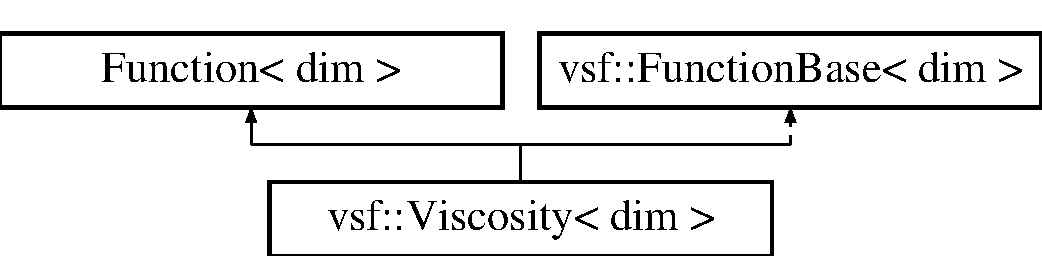
\includegraphics[height=2.000000cm]{classvsf_1_1Viscosity}
\end{center}
\end{figure}
\subsection*{Public Member Functions}
\begin{DoxyCompactItemize}
\item 
\hyperlink{classvsf_1_1Viscosity_a679e1dadfa6b003cc17f8fe9fa2bdadc}{Viscosity} ()
\item 
virtual double \hyperlink{classvsf_1_1Viscosity_adf3ee3f49d4d9695adae1f56efa69411}{value} (const Point$<$ dim $>$ \&p, const unsigned int component=0) const 
\item 
virtual void \hyperlink{classvsf_1_1Viscosity_a59d7fac27c14d4145634ed84d6ea40ee}{value\-\_\-list} (const std\-::vector$<$ Point$<$ dim $>$ $>$ \&points, std\-::vector$<$ double $>$ \&values, const unsigned int component=0) const 
\end{DoxyCompactItemize}
\subsection*{Additional Inherited Members}


\subsection{Detailed Description}
\subsubsection*{template$<$int dim$>$class vsf\-::\-Viscosity$<$ dim $>$}

The template class \hyperlink{classvsf_1_1Viscosity}{Viscosity} gives the value of the viscosity in the requested point/s 

\subsection{Constructor \& Destructor Documentation}
\hypertarget{classvsf_1_1Viscosity_a679e1dadfa6b003cc17f8fe9fa2bdadc}{\index{vsf\-::\-Viscosity@{vsf\-::\-Viscosity}!Viscosity@{Viscosity}}
\index{Viscosity@{Viscosity}!vsf::Viscosity@{vsf\-::\-Viscosity}}
\subsubsection[{Viscosity}]{\setlength{\rightskip}{0pt plus 5cm}template$<$int dim$>$ {\bf vsf\-::\-Viscosity}$<$ dim $>$\-::{\bf Viscosity} (
\begin{DoxyParamCaption}
{}
\end{DoxyParamCaption}
)\hspace{0.3cm}{\ttfamily [inline]}}}\label{classvsf_1_1Viscosity_a679e1dadfa6b003cc17f8fe9fa2bdadc}


\subsection{Member Function Documentation}
\hypertarget{classvsf_1_1Viscosity_adf3ee3f49d4d9695adae1f56efa69411}{\index{vsf\-::\-Viscosity@{vsf\-::\-Viscosity}!value@{value}}
\index{value@{value}!vsf::Viscosity@{vsf\-::\-Viscosity}}
\subsubsection[{value}]{\setlength{\rightskip}{0pt plus 5cm}template$<$int dim$>$ double {\bf vsf\-::\-Viscosity}$<$ dim $>$\-::value (
\begin{DoxyParamCaption}
\item[{const Point$<$ dim $>$ \&}]{p, }
\item[{const unsigned int}]{component = {\ttfamily 0}}
\end{DoxyParamCaption}
) const\hspace{0.3cm}{\ttfamily [virtual]}}}\label{classvsf_1_1Viscosity_adf3ee3f49d4d9695adae1f56efa69411}
\hyperlink{classvsf_1_1Viscosity_adf3ee3f49d4d9695adae1f56efa69411}{Viscosity\-::value} extracts the value in one point (\char`\"{}p\char`\"{}). In the current implementation we consider a uniform shear modulus. To use a spatially variable shear modulus modify this method accordingly. \hypertarget{classvsf_1_1Viscosity_a59d7fac27c14d4145634ed84d6ea40ee}{\index{vsf\-::\-Viscosity@{vsf\-::\-Viscosity}!value\-\_\-list@{value\-\_\-list}}
\index{value\-\_\-list@{value\-\_\-list}!vsf::Viscosity@{vsf\-::\-Viscosity}}
\subsubsection[{value\-\_\-list}]{\setlength{\rightskip}{0pt plus 5cm}template$<$int dim$>$ void {\bf vsf\-::\-Viscosity}$<$ dim $>$\-::value\-\_\-list (
\begin{DoxyParamCaption}
\item[{const std\-::vector$<$ Point$<$ dim $>$ $>$ \&}]{points, }
\item[{std\-::vector$<$ double $>$ \&}]{values, }
\item[{const unsigned int}]{component = {\ttfamily 0}}
\end{DoxyParamCaption}
) const\hspace{0.3cm}{\ttfamily [virtual]}}}\label{classvsf_1_1Viscosity_a59d7fac27c14d4145634ed84d6ea40ee}
\hyperlink{classvsf_1_1Viscosity_a59d7fac27c14d4145634ed84d6ea40ee}{Viscosity\-::value\-\_\-list} allows to extract values for several points (\char`\"{}points\char`\"{}) at once and outputs them in a vector (\char`\"{}values\char`\"{}). 

The documentation for this class was generated from the following file\-:\begin{DoxyCompactItemize}
\item 
\hyperlink{VE__fault__elastic_8cc}{V\-E\-\_\-fault\-\_\-elastic.\-cc}\end{DoxyCompactItemize}

\chapter{File Documentation}
\hypertarget{README_8md}{\section{R\-E\-A\-D\-M\-E.\-md File Reference}
\label{README_8md}\index{R\-E\-A\-D\-M\-E.\-md@{R\-E\-A\-D\-M\-E.\-md}}
}

\hypertarget{VE__fault__elastic_8cc}{\section{V\-E\-\_\-fault\-\_\-elastic.\-cc File Reference}
\label{VE__fault__elastic_8cc}\index{V\-E\-\_\-fault\-\_\-elastic.\-cc@{V\-E\-\_\-fault\-\_\-elastic.\-cc}}
}
\subsection*{Classes}
\begin{DoxyCompactItemize}
\item 
struct \hyperlink{structvsf_1_1PointHistory}{vsf\-::\-Point\-History$<$ dim $>$}
\item 
class \hyperlink{classvsf_1_1FunctionBase}{vsf\-::\-Function\-Base$<$ dim $>$}
\item 
class \hyperlink{classvsf_1_1Solution__Turcotte}{vsf\-::\-Solution\-\_\-\-Turcotte$<$ dim $>$}
\item 
class \hyperlink{classvsf_1_1Solution__Savage}{vsf\-::\-Solution\-\_\-\-Savage$<$ dim $>$}
\item 
class \hyperlink{classvsf_1_1Shear__Modulus}{vsf\-::\-Shear\-\_\-\-Modulus$<$ dim $>$}
\item 
class \hyperlink{classvsf_1_1Viscosity}{vsf\-::\-Viscosity$<$ dim $>$}
\item 
class \hyperlink{classvsf_1_1BodyForce}{vsf\-::\-Body\-Force$<$ dim $>$}
\item 
class \hyperlink{classvsf_1_1Dirichlet__BC}{vsf\-::\-Dirichlet\-\_\-\-B\-C$<$ dim $>$}
\item 
class \hyperlink{classvsf_1_1Neumann__BC}{vsf\-::\-Neumann\-\_\-\-B\-C$<$ dim $>$}
\item 
class \hyperlink{classvsf_1_1ApShear}{vsf\-::\-Ap\-Shear$<$ dim $>$}
\end{DoxyCompactItemize}
\subsection*{Namespaces}
\begin{DoxyCompactItemize}
\item 
\hyperlink{namespacevsf}{vsf}
\end{DoxyCompactItemize}
\subsection*{Functions}
\begin{DoxyCompactItemize}
\item 
int \hyperlink{VE__fault__elastic_8cc_ae66f6b31b5ad750f1fe042a706a4e3d4}{main} ()
\end{DoxyCompactItemize}


\subsection{Function Documentation}
\hypertarget{VE__fault__elastic_8cc_ae66f6b31b5ad750f1fe042a706a4e3d4}{\index{V\-E\-\_\-fault\-\_\-elastic.\-cc@{V\-E\-\_\-fault\-\_\-elastic.\-cc}!main@{main}}
\index{main@{main}!VE_fault_elastic.cc@{V\-E\-\_\-fault\-\_\-elastic.\-cc}}
\subsubsection[{main}]{\setlength{\rightskip}{0pt plus 5cm}int main (
\begin{DoxyParamCaption}
{}
\end{DoxyParamCaption}
)}}\label{VE__fault__elastic_8cc_ae66f6b31b5ad750f1fe042a706a4e3d4}
\begin{DoxyNote}{Note}
The equations are only valid for 2\-D geometries (anti-\/plane shear approximation). If the user tries to create a 3\-D geometry, an exception is thrown and the program stops.
\end{DoxyNote}
When an Ap\-Shear is created the user must specify the kind of elements and refinement (adaptive\-\_\-refinement or global\-\_\-refinement) and Model (turcotte or savage) are going oto be used.
%--- End generated contents ---

% Bibliography
\newpage
\phantomsection
\addcontentsline{toc}{chapter}{Bibliography}
\bibliographystyle{plain}
\bibliography{exportlist}

% Index
\newpage
\phantomsection
\addcontentsline{toc}{chapter}{Index}
\printindex

\end{document}
